\chapter{Рестарты зеркального спуска для липшицевых задач с условием $\gamma$-роста}\label{ch:ch3}

\section{Введение}\label{sec:ch3/sect1}

    Широко известно, что негладкие оптимизационные задачи обладают пессимистичными теоретическими оценками скорости сходимости в пространствах больших размерностей. Одним из подходов к этой проблеме может служить выделение специального класса задач с условием острого минимума \cite{6, 1} и дальнейшее развитие данного условия. Говорят, что $f$ удовлетворяет условию острого минимума, если
    \begin{gather}\label{sm}
    f(x) - f(x_*) \geq \alpha \min_{x_* \in X_*} \|x- x_*\|_2 \quad \forall x \in Q
    \end{gather}
    для некоторого фиксированного $\alpha >0$ и $f(x_*) = f^* = \min\limits_{x\in Q} f(x)$ для всякого $x_* \in X_*$, где $Q$ --- выпуклое и замкнутое подмножество $\mathbb{R}^n$, $X_*$ --- компакт и $\|\cdot\|_2$ --- евклидова норма. 
    При таком допущении моими соавторами был предложен субградиентный метод с гарантией  линейной скорости сходимости в случае доступности информации о точном значении $f^*$ \cite{6} без использования в теоретических оценках скорости сходимости  параметра размерности пространства. Условие острого минимума верно, например, для задачи проектирования точки на выпуклый компакт. Однако требование доступности $f^*$ довольно ограничительно. В этой связи рассматривалось некоторое обобщение условия острого минимума
    \begin{gather}\label{eq_gen_sharp}
    f(x) - \overline{f} \geq \alpha \min_{x_* \in X_*} \|x - x_* \|_2 - \Delta,
    \end{gather}
    где $\overline{f}$  --- это некоторое приближение минимального значения функции $f^*$, причём $\overline{f} \geq f^*$. Такое обобщение позволяет несколько расширить класс применимости субградиентных методов для задач с острым минимумом и шагом Б.Т. Поляка. Например, оно может покрыть постановку задачи с неточной информацией о $f^*$.  

    В данной главе предложен анализ проведенного экспериментального сравнения двух субградиентных методов, использующих различные дополнительные условия:
    \begin{enumerate}
        \item сильной выпуклости,
        \item обобщенного условия острого минимума.
    \end{enumerate}
    Также, на основе проведенного противопоставления указанных выше условий, предложены рестарты для субградиентных методов, улучшающие полученные ранее оценки благодаря использованию аналога условия острого минимума.  Кроме того, предложена некоторая релаксация для понятия острого минимума, включающая в себя условие квадратичного роста и использующая функцию Брегмана для оценки удаленности от решения. 

\section{Адаптивная оценка скорости сходимости одного субградиентного метода для сильно выпуклых задач и вычислительные эксперименты для задачи о наименьшем покрывающем шаре}  \label{sec:ch3/sec2}

    В предыдущей главе были доказаны сублинейные оценки для достаточно широкого класса задач. Однако сублинейная скорость сходимости значительно уступает передовым результатам для задач, обладающих сильной выпуклостью. Альтернативным направлением развития субградиентых методов является использование условия острого минимума, для которого моими соавторами в работе [] была доказана соответствующая теорема [].\\  
    Напомним, что в работе рассматриваются задачи вида
    \begin{gather}\label{min_q}
        f(x)\rightarrow\min_{x\in Q},
    \end{gather}
    где $Q$ --- выпуклое замкнутое подмножество $\mathbb{R}^{n}$. Для субградиентного метода вида
    \begin{gather}\label{orig}
        x_{k+1} := Pr_{Q}\{x_k - h_k \nabla f(x_k) \}, \;\; \textit{где} \; h_k = \frac{2}{\mu (k+1)}
    \end{gather}

    Приведем без доказательства результат, полученный моими коллегами, который необходим для дальнейшего анализа экспериментально полученных результатов.
    \begin{theorem}\label{theorem1}
        Пусть $f$ --- слабо $\beta$-квазивыпуклая функция и для задачи \eqref{min_q} с условием \eqref{eq_gen_sharp} используется метод \eqref{orig} c шагом
        $h_k = \dfrac{\beta(f(x_k) - \overline{f})}{\| \nabla f(x_k) \|_2^2}$. Пусть также $\forall i \geq 0$ верно $\alpha^2 \beta^2 \leq 2 \| \nabla f(x_i) \|_2^2$. Тогда верно неравенство:
        \begin{gather}\label{adaptive_estimate}
            \begin{aligned}
            \min_{x_* \in X_*} \|x_{k+1} - x_* \|_2^2 \leq &  \prod_{i=0}^k \left ( 1 - \frac{\alpha^2\beta^2}{2 \| \nabla f(x_i) \|_2^2} \right ) \min_{x_* \in X_*} \|x_0 - x_* \|_2^2 + \\& 
            \qquad \qquad + \sum_{i=0}^{k-1} \prod_{j=i+1}^k \left ( 1 - \frac{\alpha^2\beta^2}{2 \| \nabla f(x_j) \|_2^2} \right )\Delta_i + \Delta_k,
            \end{aligned}
        \end{gather}
        где $\Delta_k = \frac{\Delta^2}{2 \| \nabla f(x_k) \|_2^2}$ для всякого $k \geqslant 0$.
    \end{theorem}

    Для сравнения воспользуемся улучшенной версией следующей оценки скорости сходимости \cite{Bach_2012}:
    \begin{equation}\label{orig_estimation_f}
        f(\widehat{x}) - f(x_*) \leq \frac{2 M^2}{\mu (N+1)}  \; \text{  при   } \; \widehat{x} = \sum\limits_{k=1}^{N} \frac{2 k}{N (N+1)} x_k, 
    \end{equation}
    где $M$ --- константа Липщица целевой функции $f$.

    Данную оценку можно несколько улучшить на классе сильно выпуклых задач, что было описано в \cite{Stonyakin_2021}. Воспользуемся рассуждением, проведенным для вариационных неравенств в замечании \ref{remark4} и приведем соответствующий известный результат:
    \begin{theorem}\label{ThmBachAdaptive}
        Пусть $f$ --- $\mu$-сильно выпуклая функция. Тогда после $N$ итераций алгоритма:
        $$
            x_{k+1} := Pr_{Q}\{x_k - h_k \nabla f(x_k) \}, \;\; \textit{где} \; h_k = \frac{2}{\mu (k+1)}
        $$
        будет верно неравенство:
        \begin{equation}\label{adaptive_estimation_f}
            f(\widehat{x}) - f(x_*) \leq \frac{2}{\mu N (N+1)} \sum_{k=1}^{N} \frac{k \|\nabla f(x_k)\|_2^2}{k+1},
        \end{equation}
        где
        $$
            \widehat{x} = \sum_{k=1}^{N} \frac{2 k}{N (N+1)} x_k.
        $$
        Если $f$ ещё и $M$-липшицева при $M >0$, то
        $$
             f(\widehat{x}) - f(x) \leq \varepsilon
        $$
        после $N = \mathcal{O}(\frac{M^2}{\mu\varepsilon})$ итераций алгоритма \eqref{orig}.
    \end{theorem}

    Отметим, что если $x_*$ --- точное решение задачи минимизации $f$, то можно получить оценку скорости сходимости по аргументу вида
    \begin{equation} \label{arg_est}
        \|\widehat{x} - x_*\|_2 \leq \frac{4}{\mu N (N+1)} \sum_{k=1}^{N} \frac{k \|\nabla f(x_k)\|_2^2}{k+1} \leq \frac{4M^2}{\mu(N+1)}.
    \end{equation}

    Полученный в теореме \ref{ThmBachAdaptive} результат применим и в случаях, когда константа Липщица ($M$) --- бесконечна или её значение сложно оценить. Более того, данный подход может быть распространён на важные прикладные задачи, среди которых задача бинарной классификации методом опорных векторов (SVM) \cite{Bach_2012}. По аналогии с работой \cite{Bach_2012} можно применять стохастический вариант зеркального спуска \eqref{orig}. Также отметим, что данные рассуждения и метод аналогичны описанным в предыдущей главе обобщениям на класс вариационных неравенств, лагранжевых и седловых задач. 

    Для сравнения скорости сходимости метода \cite{Bach_2012} и полученной в теореме \ref{ThmBachAdaptive} оценки с результатом, полученным моими соавторами, в теореме \ref{theorem1} для задач с $\Delta$-острым минимумом проведены численные эксперименты для задачи о наименьшем покрытии точек шаром для $2$-сильно выпуклой функции
    \begin{gather}\label{sphere_cover_strongly}
        f(x) := \max_{x\in Q}\left\{\|x - a_0\|_2^2, \|x - a_1\|_2^2, ..., \|x - a_m\|_2^2\right\},
    \end{gather}
    а также для не сильно выпуклой (но выпуклой) функции
    \begin{gather}\label{sphere_cover}
        f(x) := \max_{x\in Q}\left\{\|x - a_0\|_2, \|x - a_1\|_2, ..., \|x - a_m\|_2\right\}.
    \end{gather}

    Начнём с иллюстрации преимуществ адаптивной оценки метода \cite{Bach_2012} из теоремы \ref{ThmBachAdaptive}. Будем рассматривать множество Q, которое равно евклидову шару с центром в 0. Начальная точка выбиралась случайно, но внутри Q. На рис. \ref{res_ex_strong_r5} ниже показано поведение и характер убывания для оригинальной оценки (\ref{orig_estimation_f}) --- сплошная линия, адаптивной оценки (\ref{adaptive_estimation_f}) --- штрих-пунктирная линия и непосредственно невязки по функции и по аргументу соответственно --- штриховая линия. На рис. \ref{res_ex_strong_r5} показано поведение глобальной оценки, адаптивной и невязки по функции и аргументу в случае ограниченного $Q (R = 5)$. Данный график наглядно демонстрирует, насколько более точной может оказаться адаптивная оценка (\ref{adaptive_estimation_f}) для задачи \eqref{sphere_cover_strongly}. 

    \begin{figure}[h]
        \minipage{0.49\textwidth}
        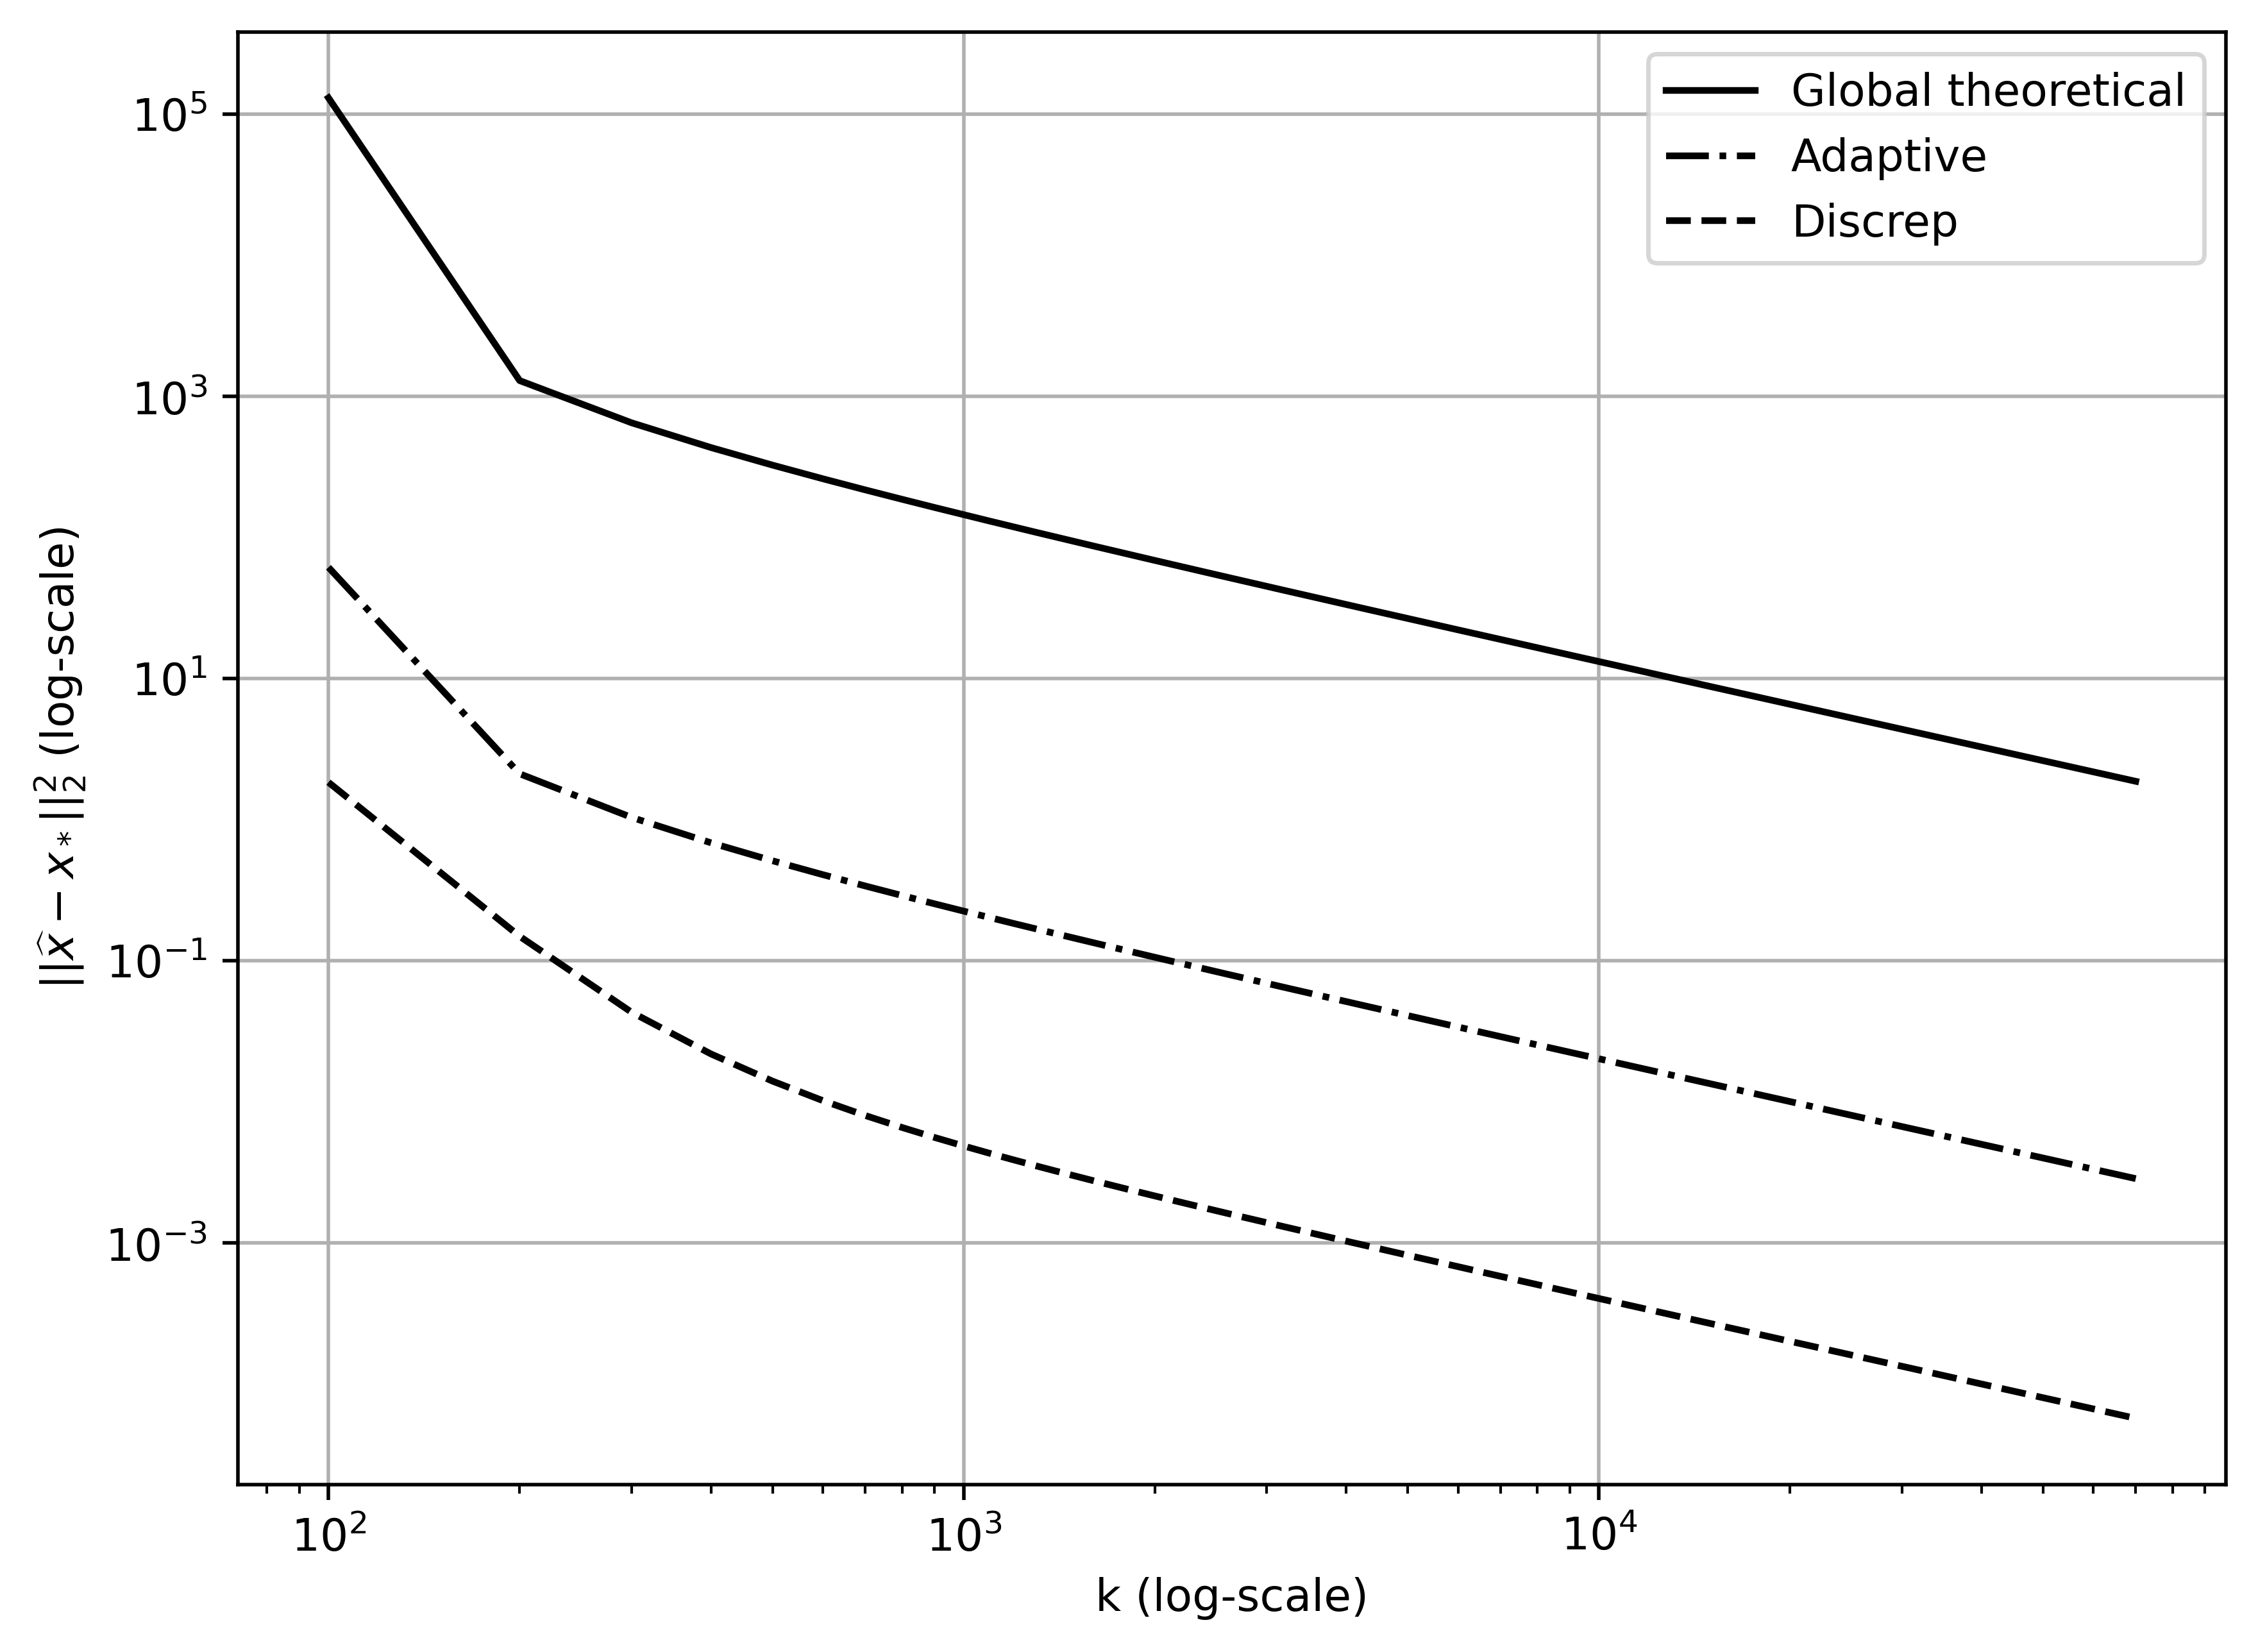
\includegraphics[width=\linewidth]{x_discr_rad_5_q_4_it_70_000_dim_1000.png}
        \endminipage\hfill
        \minipage{0.49\textwidth}
        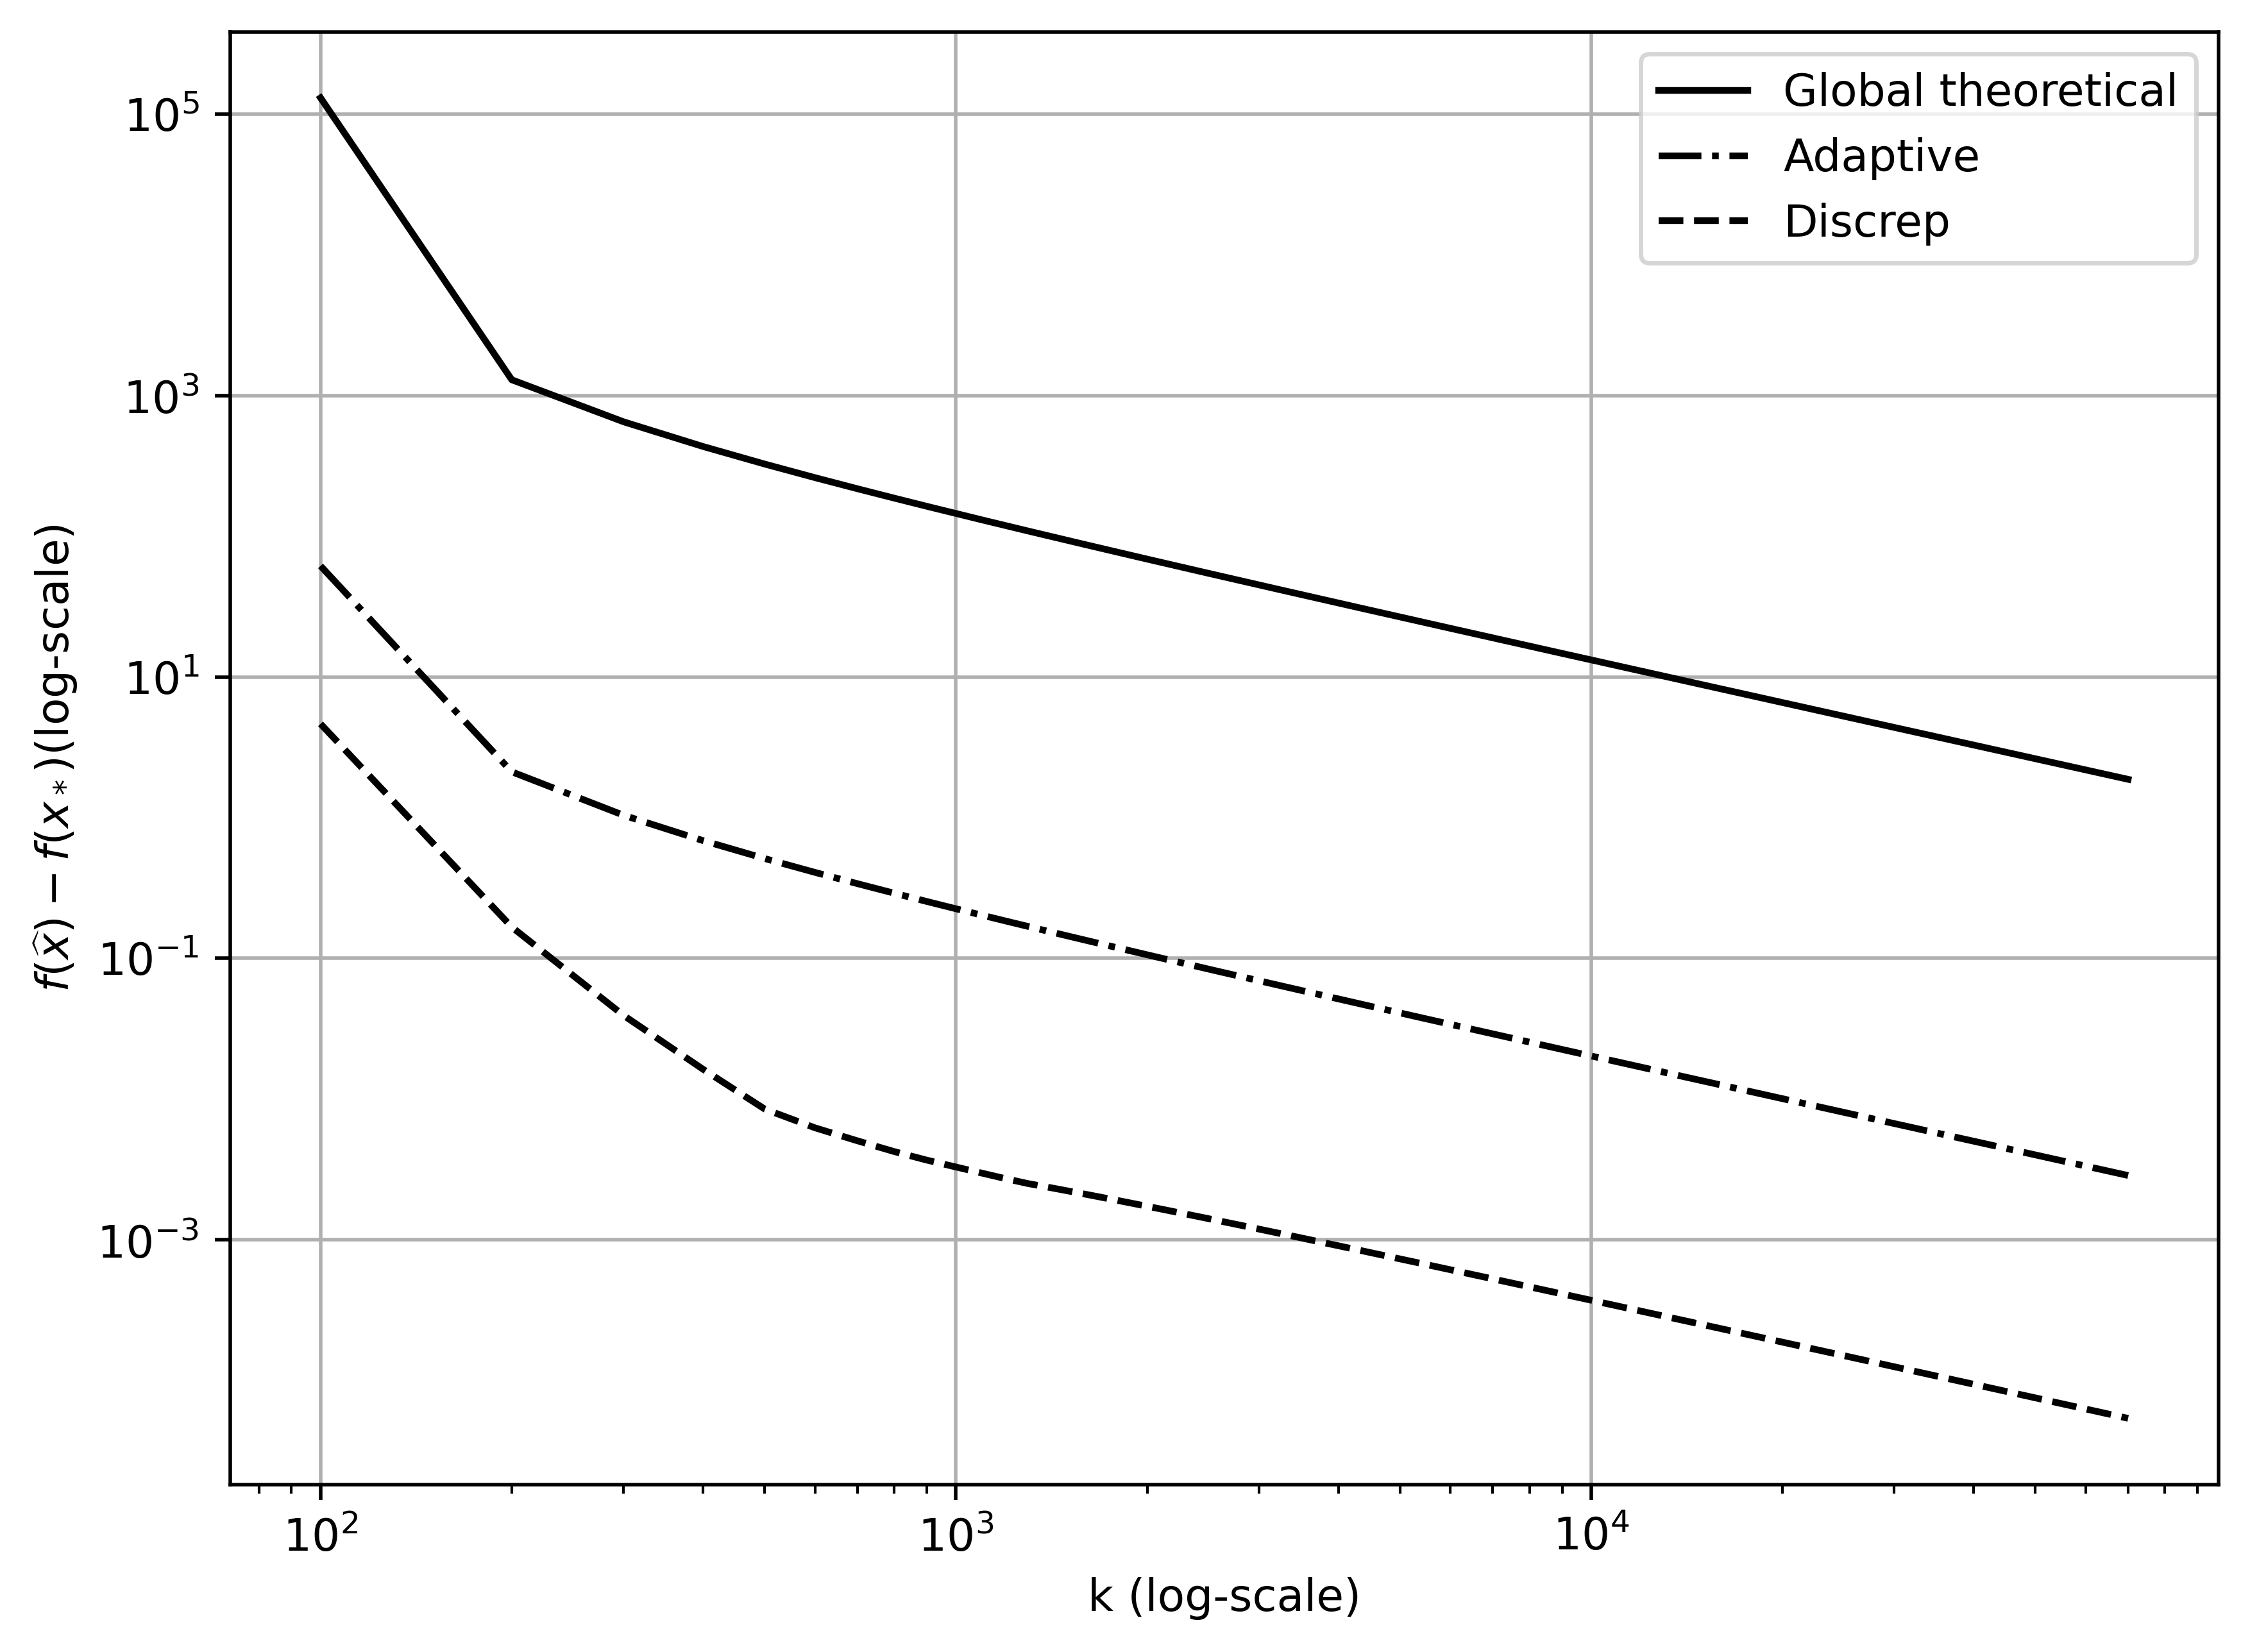
\includegraphics[width=\linewidth]{f_discr_rad_5_q_4_it_70_000_dim_1000.png}
        \endminipage\hfill
        \caption{Результаты решения задачи минимизации \eqref{sphere_cover_strongly}, где  $n= 1\,000, r = 5$ и  шар $Q$ радиуса 4.}
        \label{res_ex_strong_r5}
    \end{figure}

    Теперь перейдём к выпуклой постановке \eqref{sphere_cover} с целью исследования эффективности предложенного в теореме \ref{theorem1} субградиентного метода с $\Delta$-острым минимумом. К существующему набору точек, представленных для покрытия, с известным значением центра добавим дополнительную точку, которая находится вне исходного шара достаточно близко к границе (удалена не более, чем на $\Delta > 0$). Данный подход позволяет оценить <<приближённое>> значение минимума $\overline{f}$, что позволит применить указанный вариант субградиентного метода с $\Delta$-острым минимумом. При этом новое значение минимума останется внутри исходной сферы. Поскольку оптимальное значение функции --- это радиус искомого шара, покрывающего все точки, а $x_*$ всегда будет расположена внутри него, то для всякого $x$ верно неравенство $ f(x) \geq \| x - x_*\|_2$. Рассмотрим целевую функцию вида
    \begin{gather}\label{allpha_sphere_cover}
        f(x) := \alpha \max_{x\in Q}\{\|x - a_0\|_2, \|x - a_1\|_2, ..., \|x - a_m\|_2\}.
    \end{gather}
    Тогда значение $\Delta$ можно оценить  из (\ref{eq_gen_sharp}): 
        $f(x) - \overline{f} \geq \alpha\|x- x_*\|_2 - \Delta, \quad \Delta \geq \overline{f}$.

    Отметим, что данная постановка значительно влияет на величину теоретической оценки качества решения (\ref{adaptive_estimate}) для метода \eqref{orig}.
    Наиболее значимый вклад в оценку (\ref{adaptive_estimate}) дает последнее слагаемое $\frac{\Delta^2}{2\|\nabla f(x_k)\|^2_2}$, причём 
    $     \Delta \sim \overline{f} \sim \alpha \|\overline{x}-a\|_2 $ и 
    $     \|\nabla f(x_k)\|_2 = \alpha $. Поэтому последнее слагаемое пропорционально радиусу шара, соответствующему <<приближённому>> решению. Это и подтверждается экспериментально. Для сравнения, ниже на рис. \ref{res_sharp_convex} и \ref{res_strong_convex} приведены результаты работы для того же набора входных точек, которые необходимо покрыть в обоих постановках --- (\ref{allpha_sphere_cover}) и (\ref{sphere_cover_strongly}). Начальная точка также одна и та же. Сравниваются методы из теоремы \ref{theorem1} и \eqref{orig}. Первый из этих методов обеспечивает сходимость буквально за 10 итераций к <<приближённому>> решению с заданной точностью и даже позволяет эту точность повысить. Второй же метод достигает схожих (с геометрической точки зрения) результатов за значительно большее количество итераций, однако он позволяет повышать точность приближённого решения на дальнейших итерациях.

    Подтверждение данного теоретического наблюдения хорошо иллюстрируется на рис. \ref{res_sharp_convex} и \ref{res_strong_convex}. На рис. \ref{res_sharp_convex} показано поведение субградиентного спуска, использующего $\Delta$-острый минимум (теорема \ref{theorem1}), а именно --- быстрая сходимость к <<приближенному>> решению. Штрих-пунктирная линия соответствует оценке \eqref{eq_gen_sharp}, а штриховая --- невязке по функции и аргументу. На рис. \ref{res_strong_convex} показано поведение метода для той же задачи, но с использованием сильно выпуклого целевого функционала (теорема \ref{ThmBachAdaptive}). Скорость убывания уже не столь высокая, но точность получаемого решения в итоге выше. Сплошная линия --- это глобальная оценка \eqref{orig_estimation_f}, штрих-пунктирная --- адаптивная \eqref{adaptive_estimation_f}, а штриховая --- невязка по функции и аргументу.

    \begin{figure}[h]
        \minipage{0.49\textwidth}
        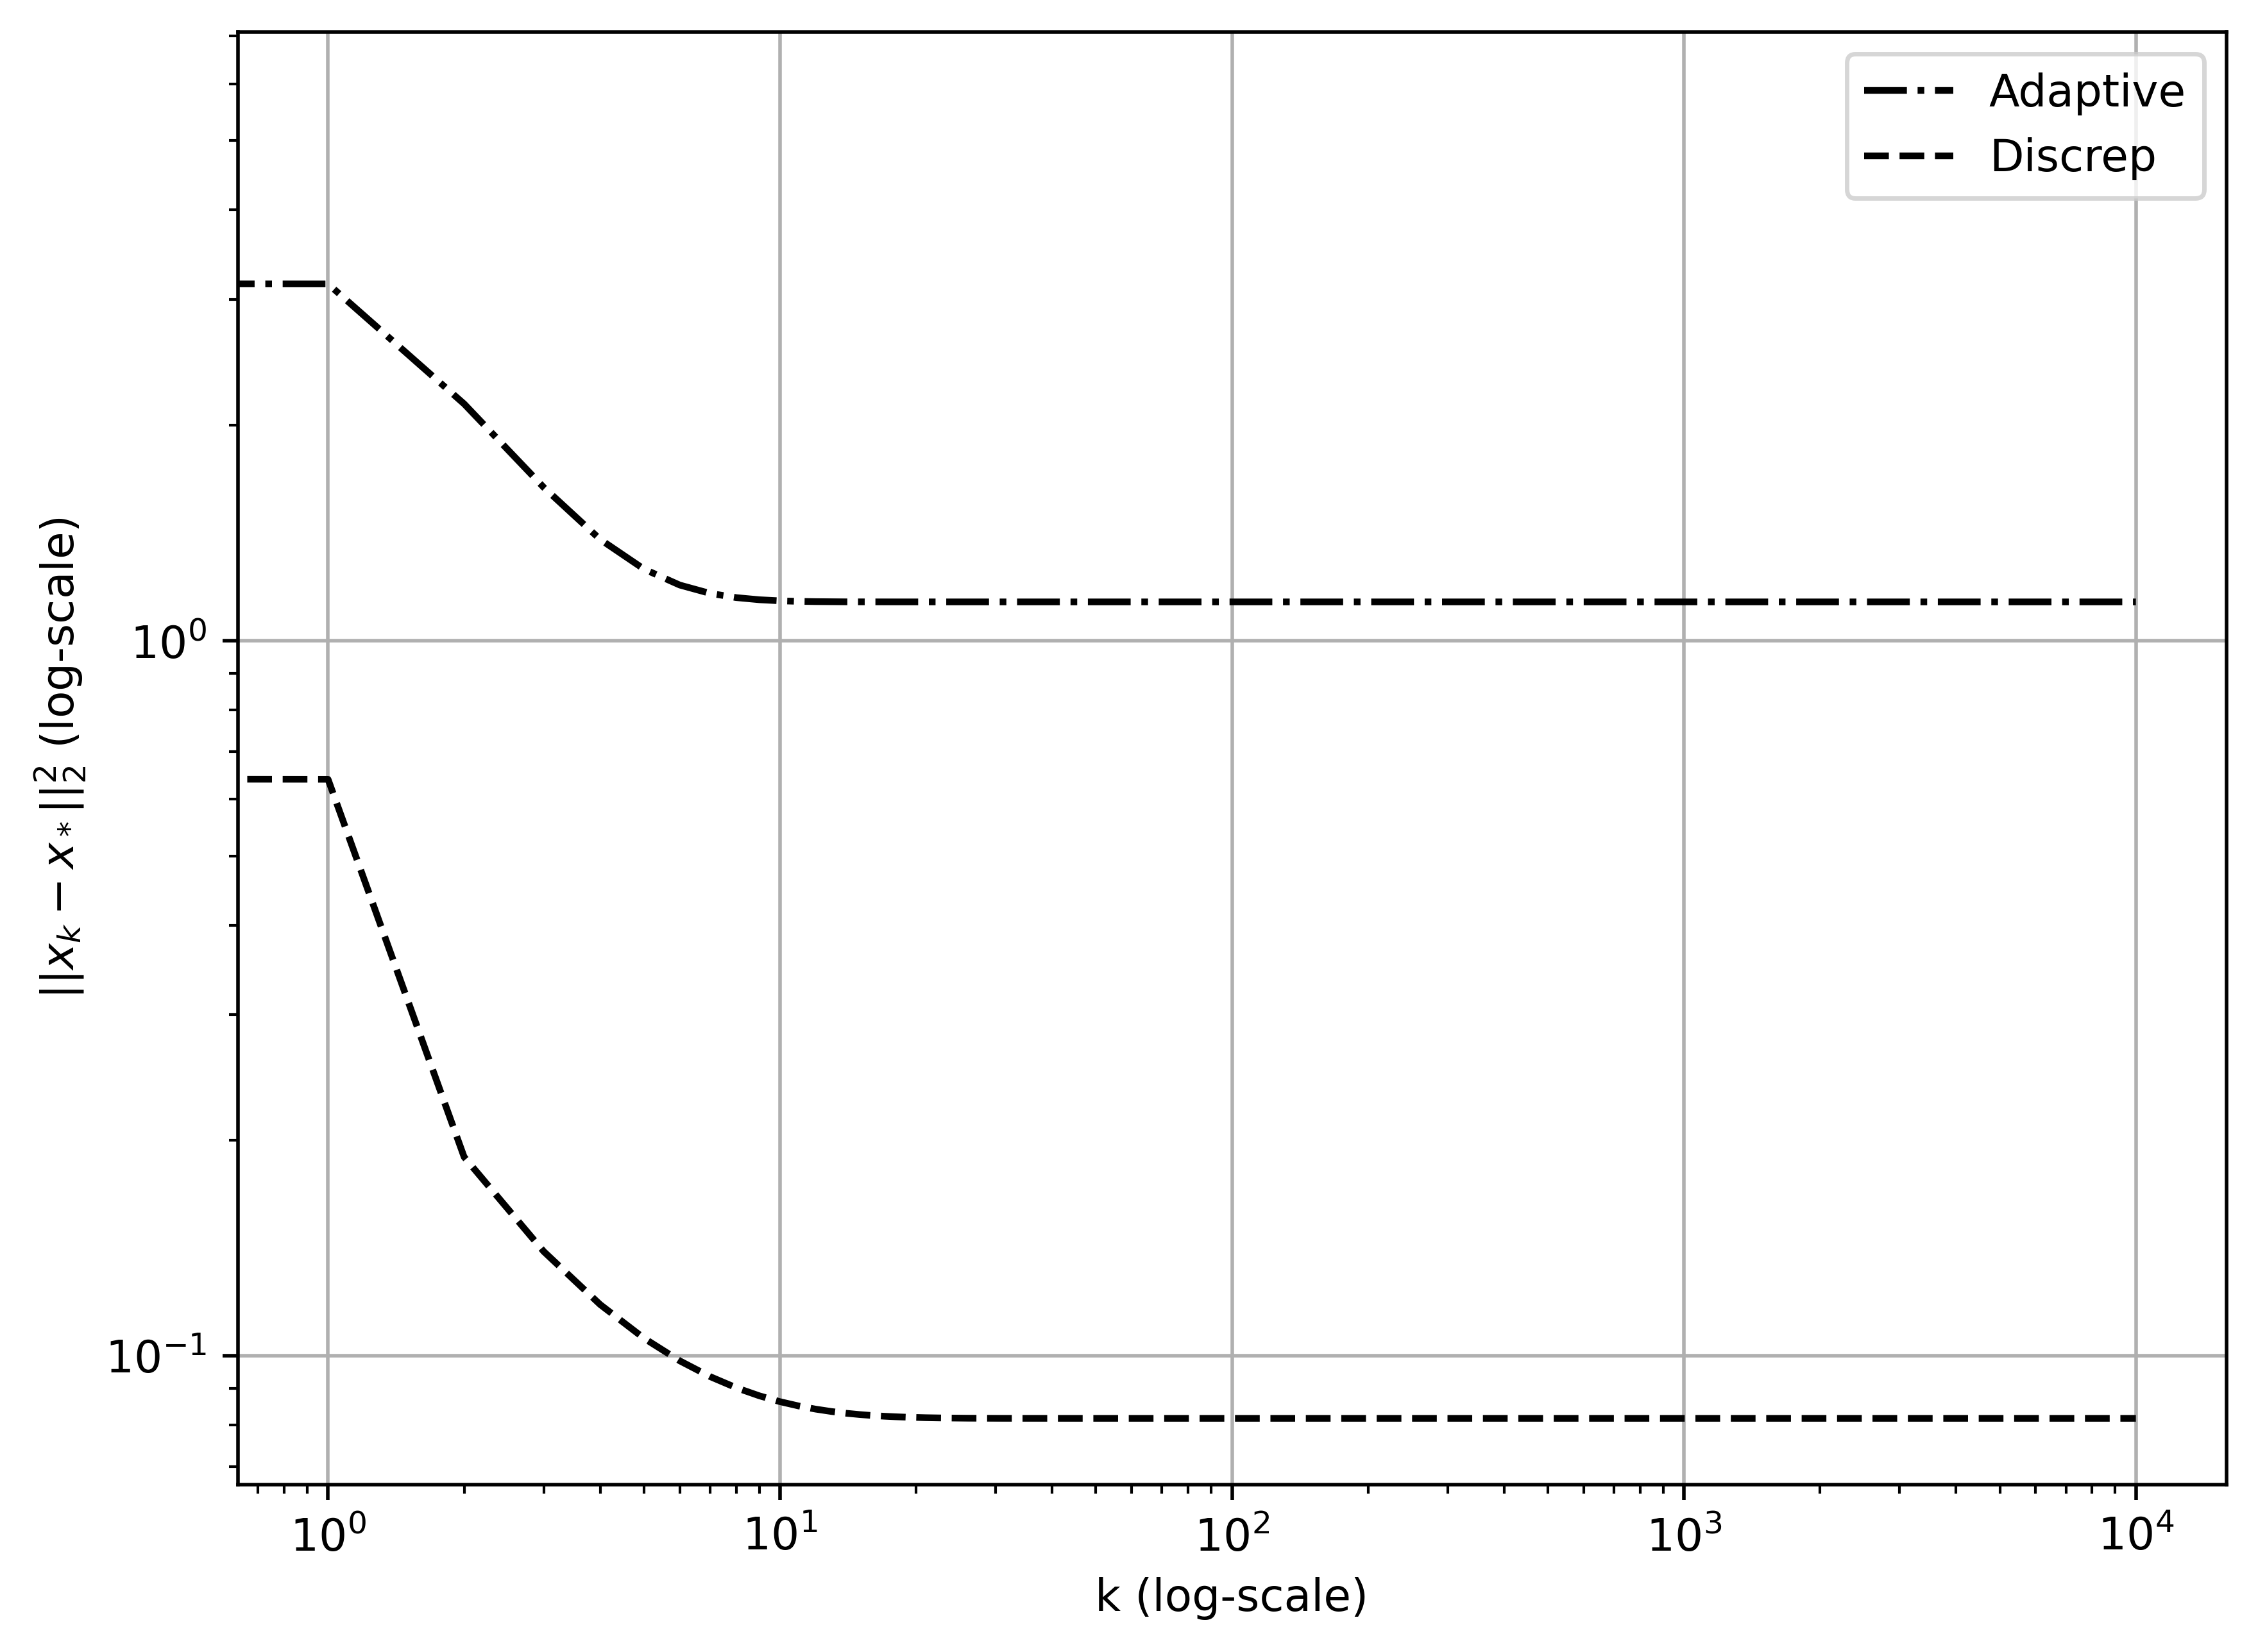
\includegraphics[width=\linewidth]{sharp_convex_x.png}
        \endminipage\hfill
        \minipage{0.49\textwidth}
        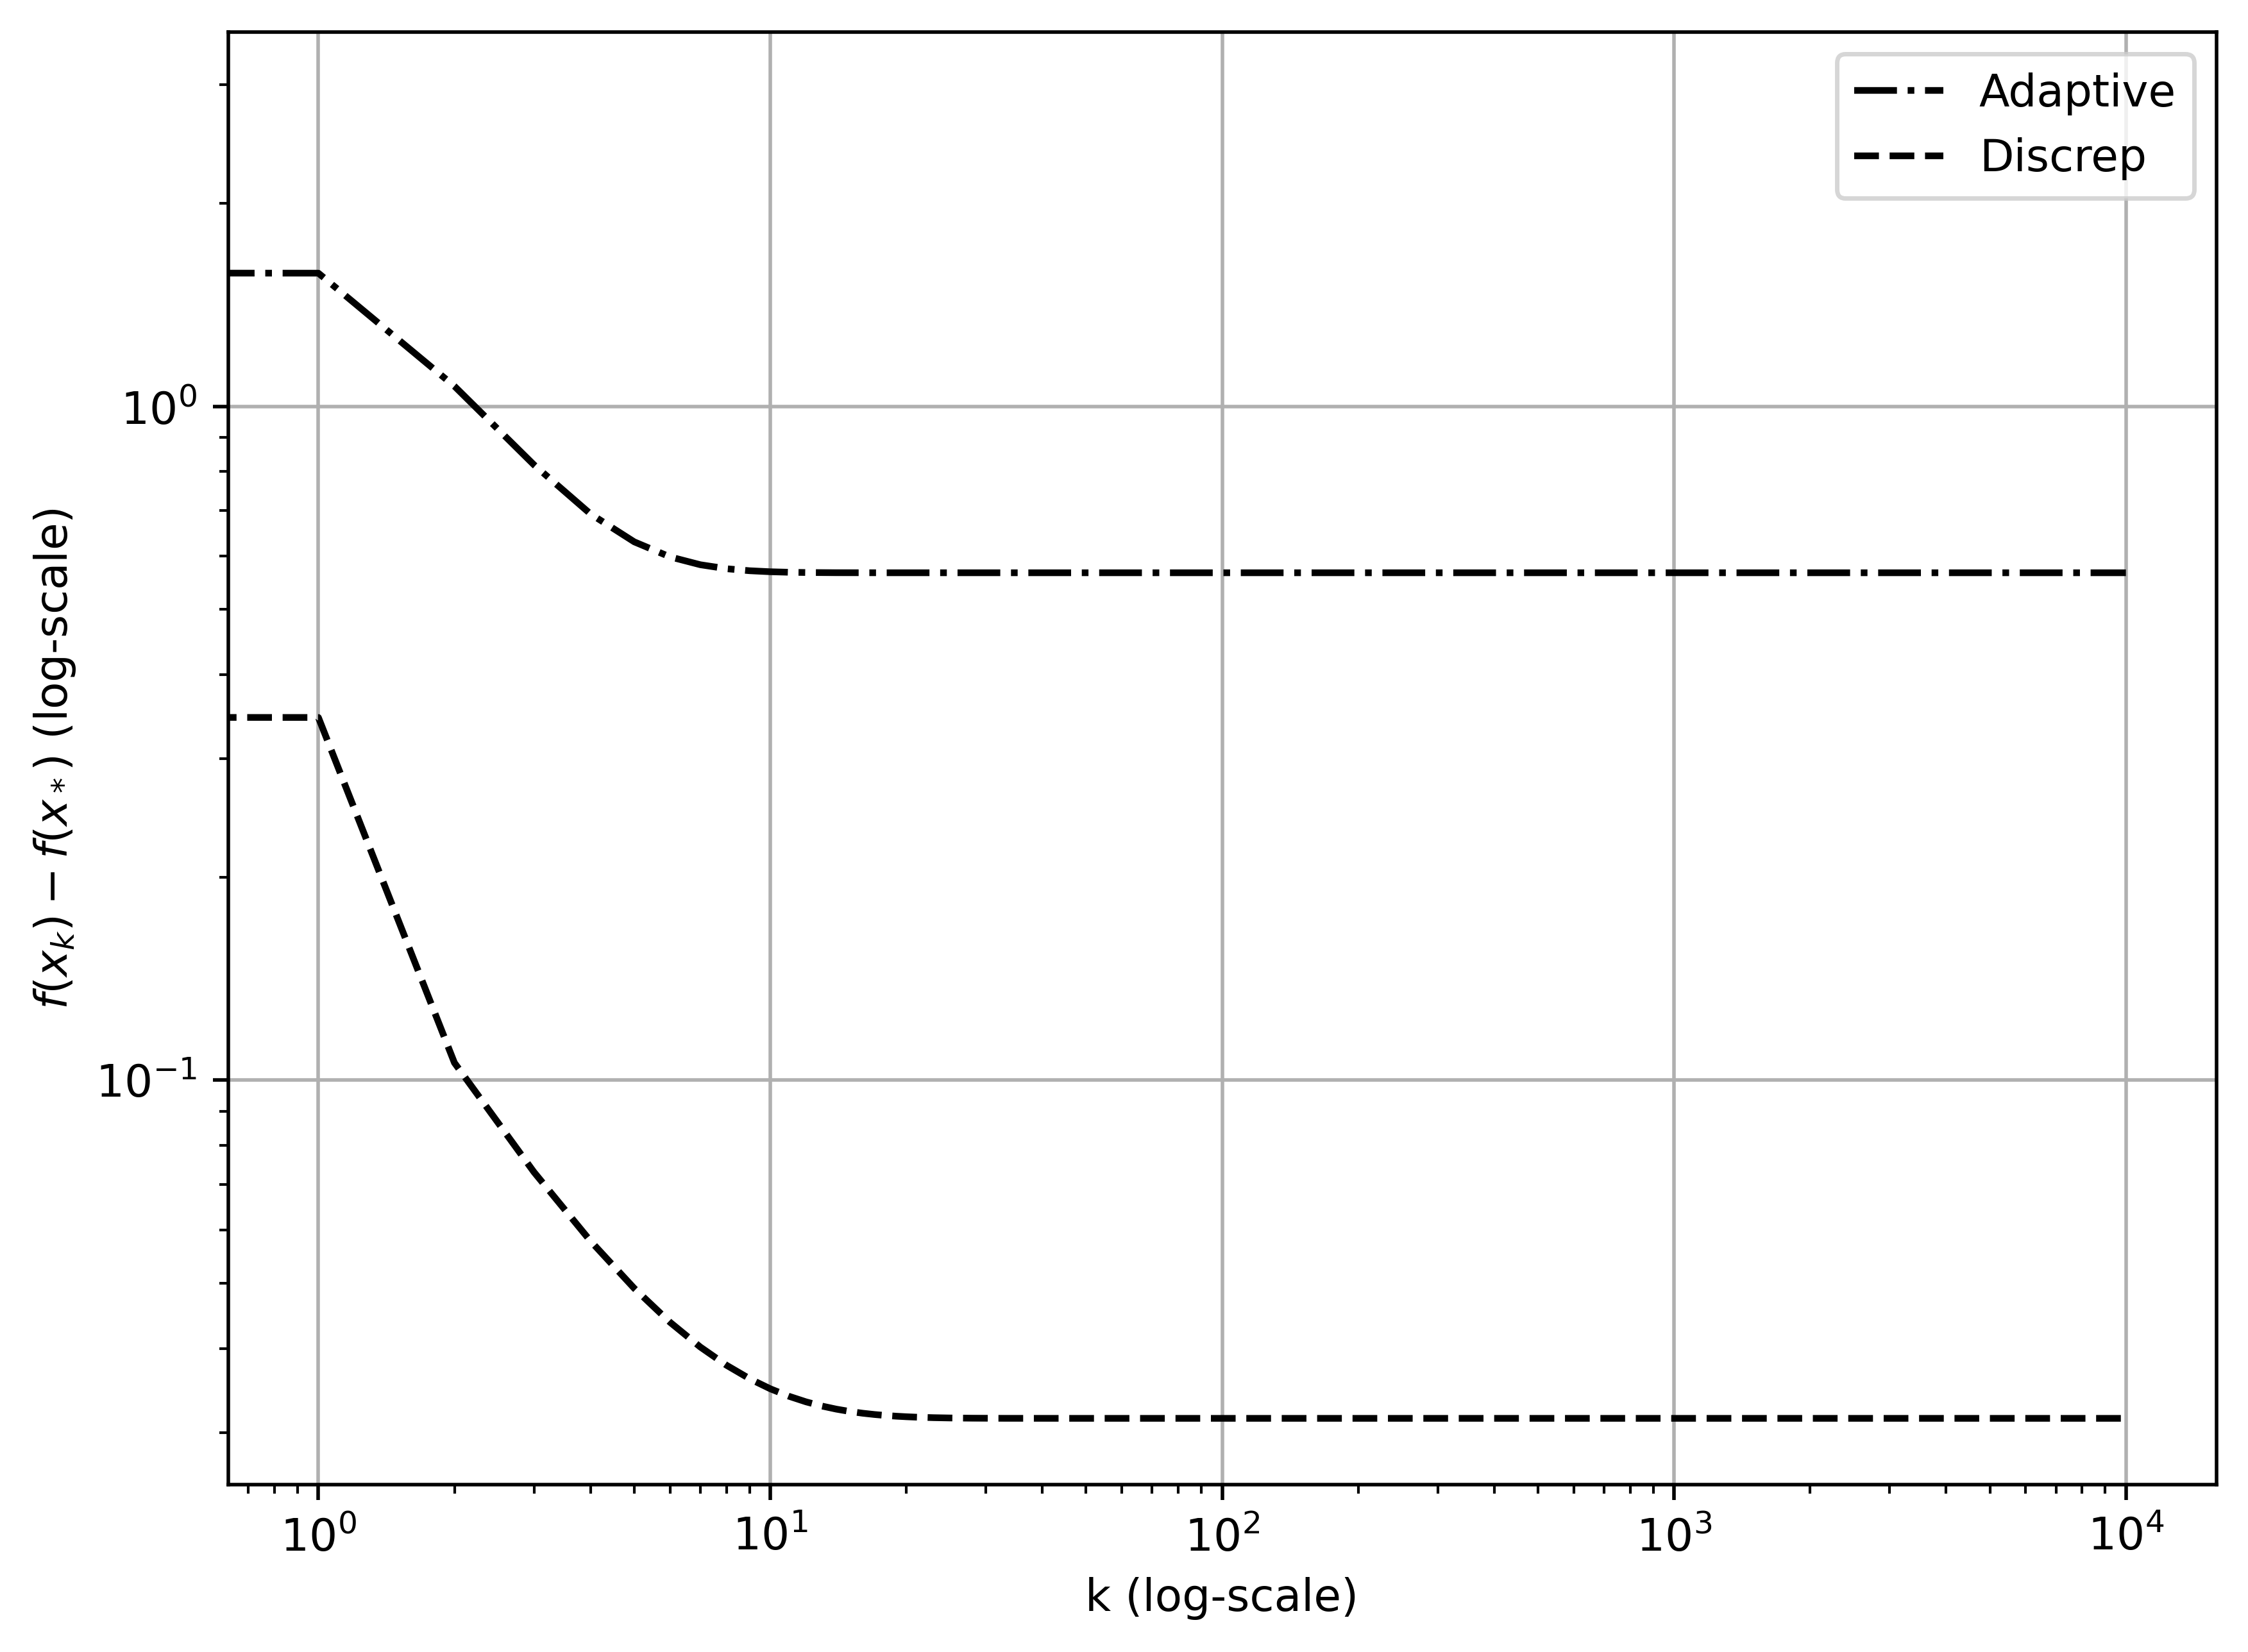
\includegraphics[width=\linewidth]{sharp_convex_f.png}
        \endminipage\hfill
        \caption{ Результаты решения задачи минимизации (\ref{allpha_sphere_cover}), где  $n= 1\,000, r = 0.7525, \alpha = 0.6$.}
        \label{res_sharp_convex}
    \end{figure}

    \begin{figure}[h]
        \minipage{0.49\textwidth}
        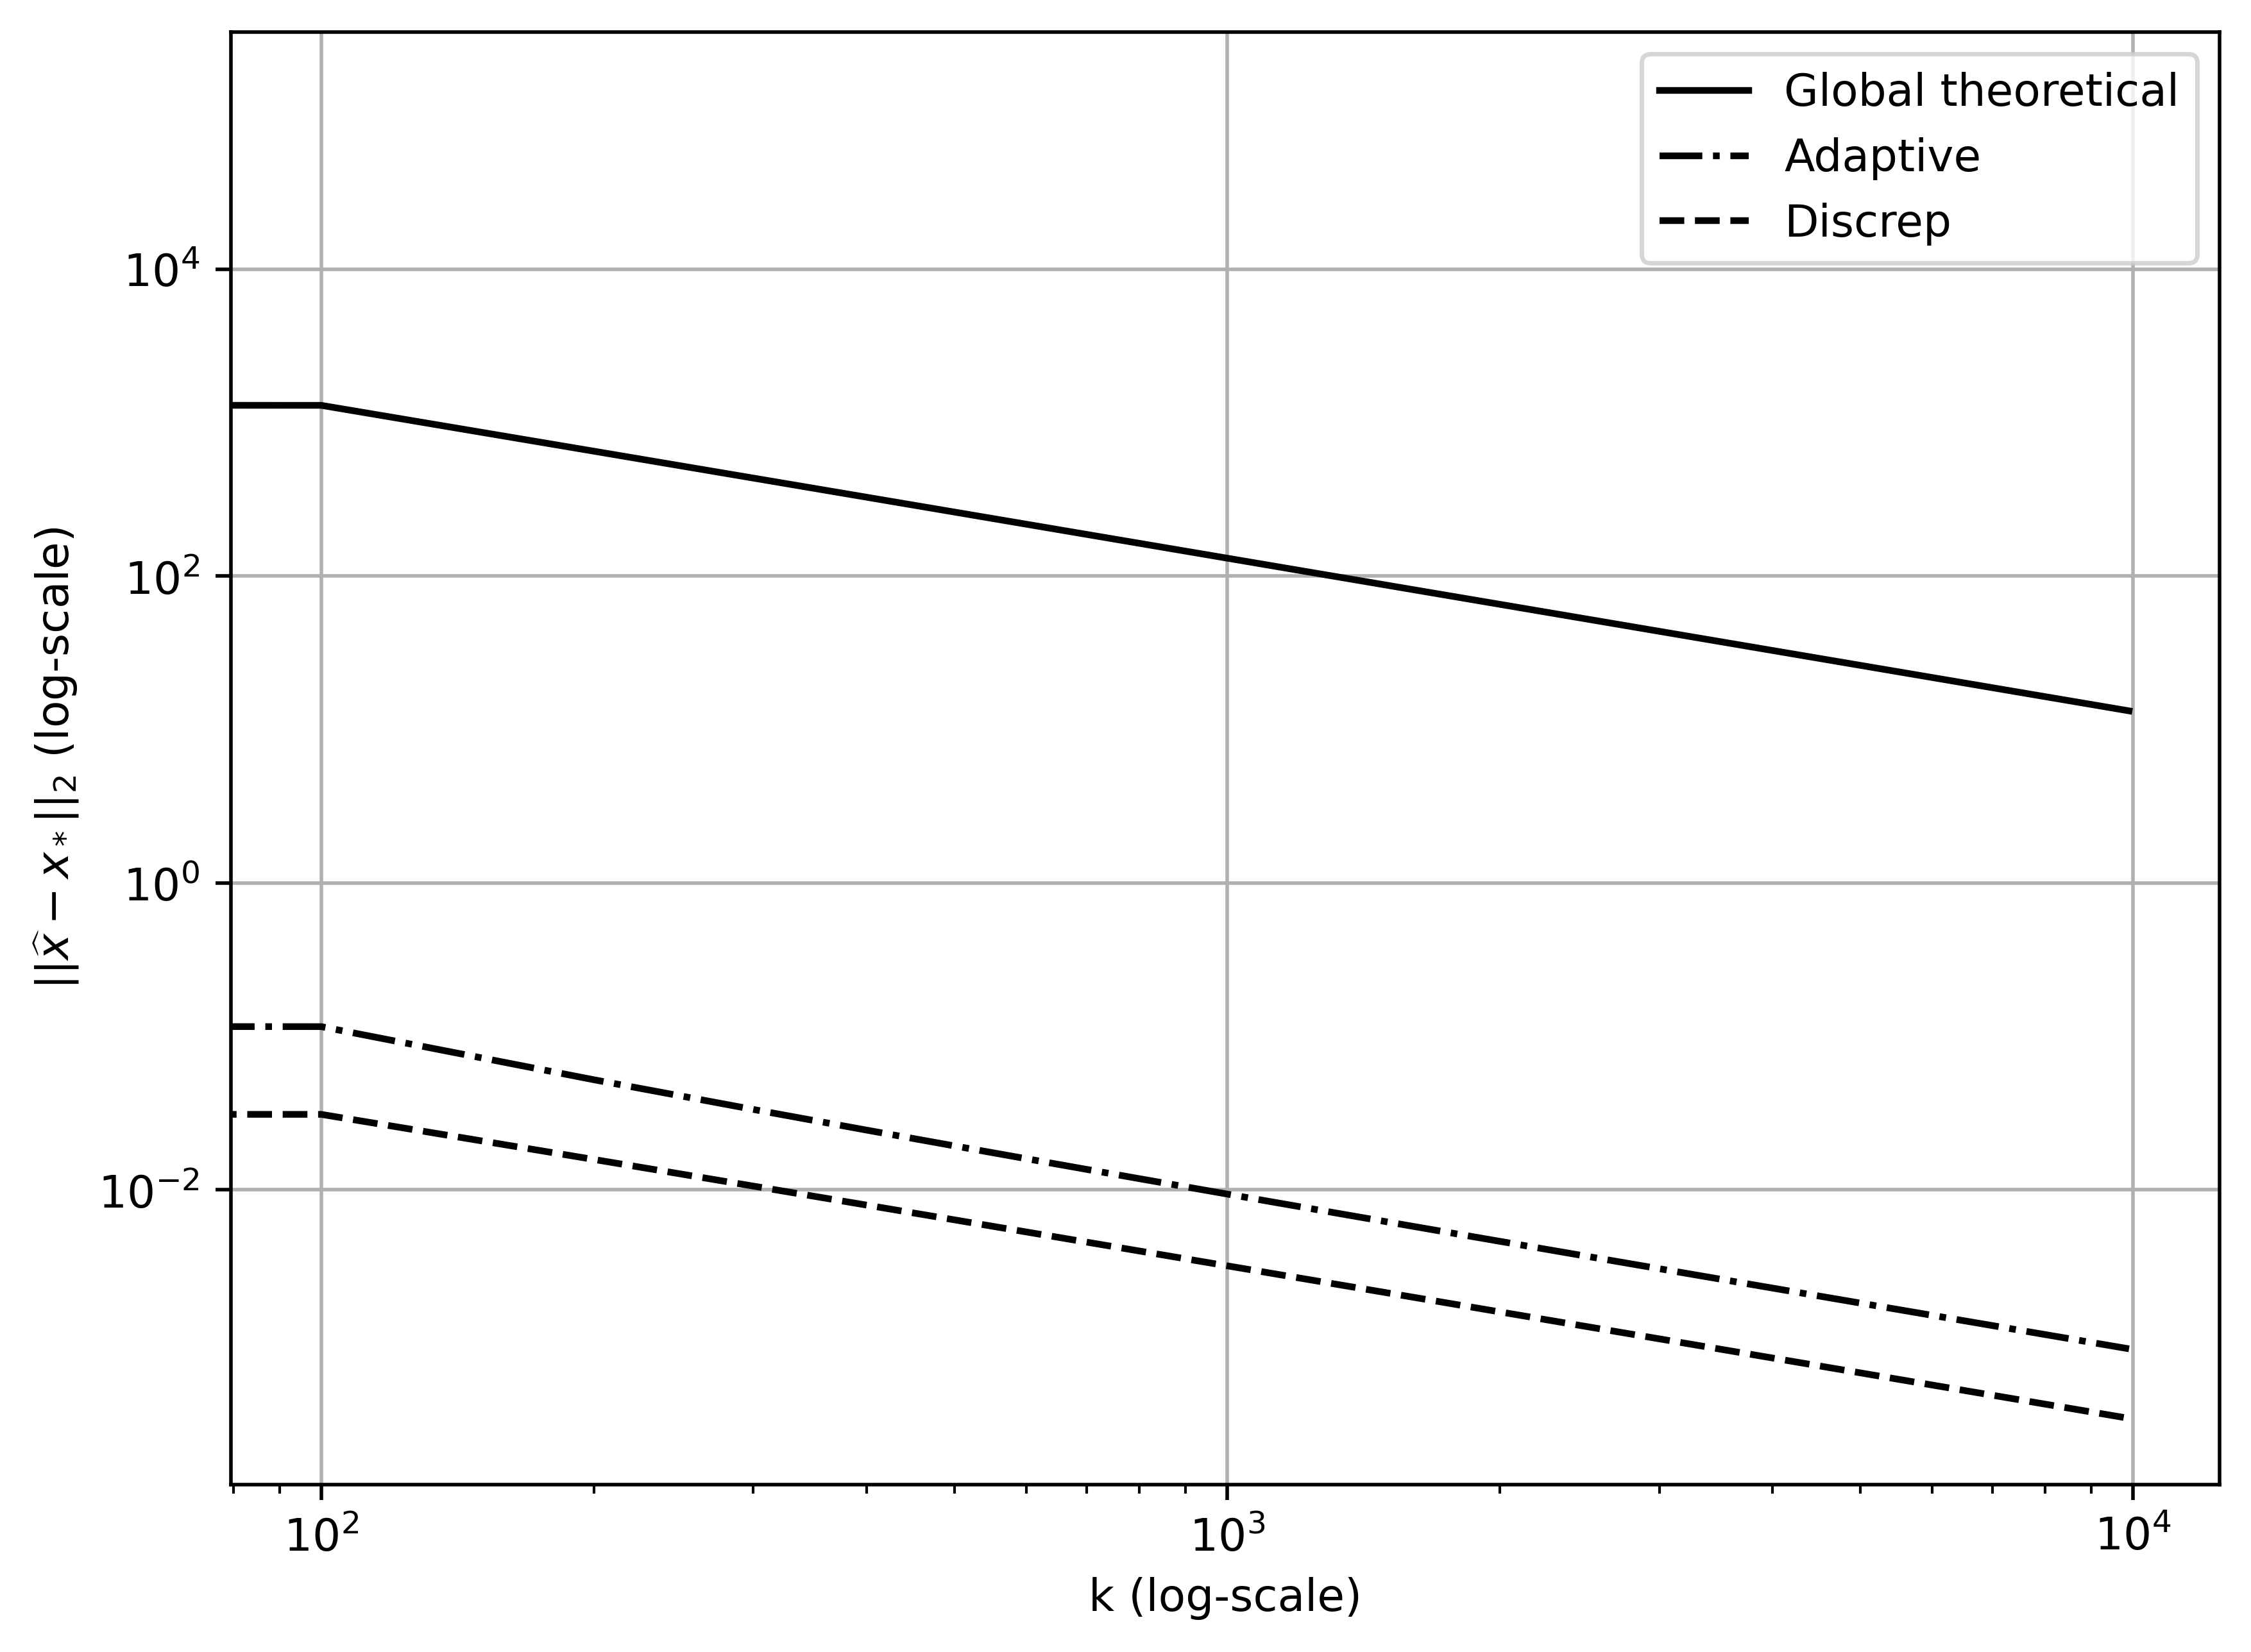
\includegraphics[width=\linewidth]{strong_convex_small_rad_x.png}
        \endminipage\hfill
        \minipage{0.49\textwidth}
        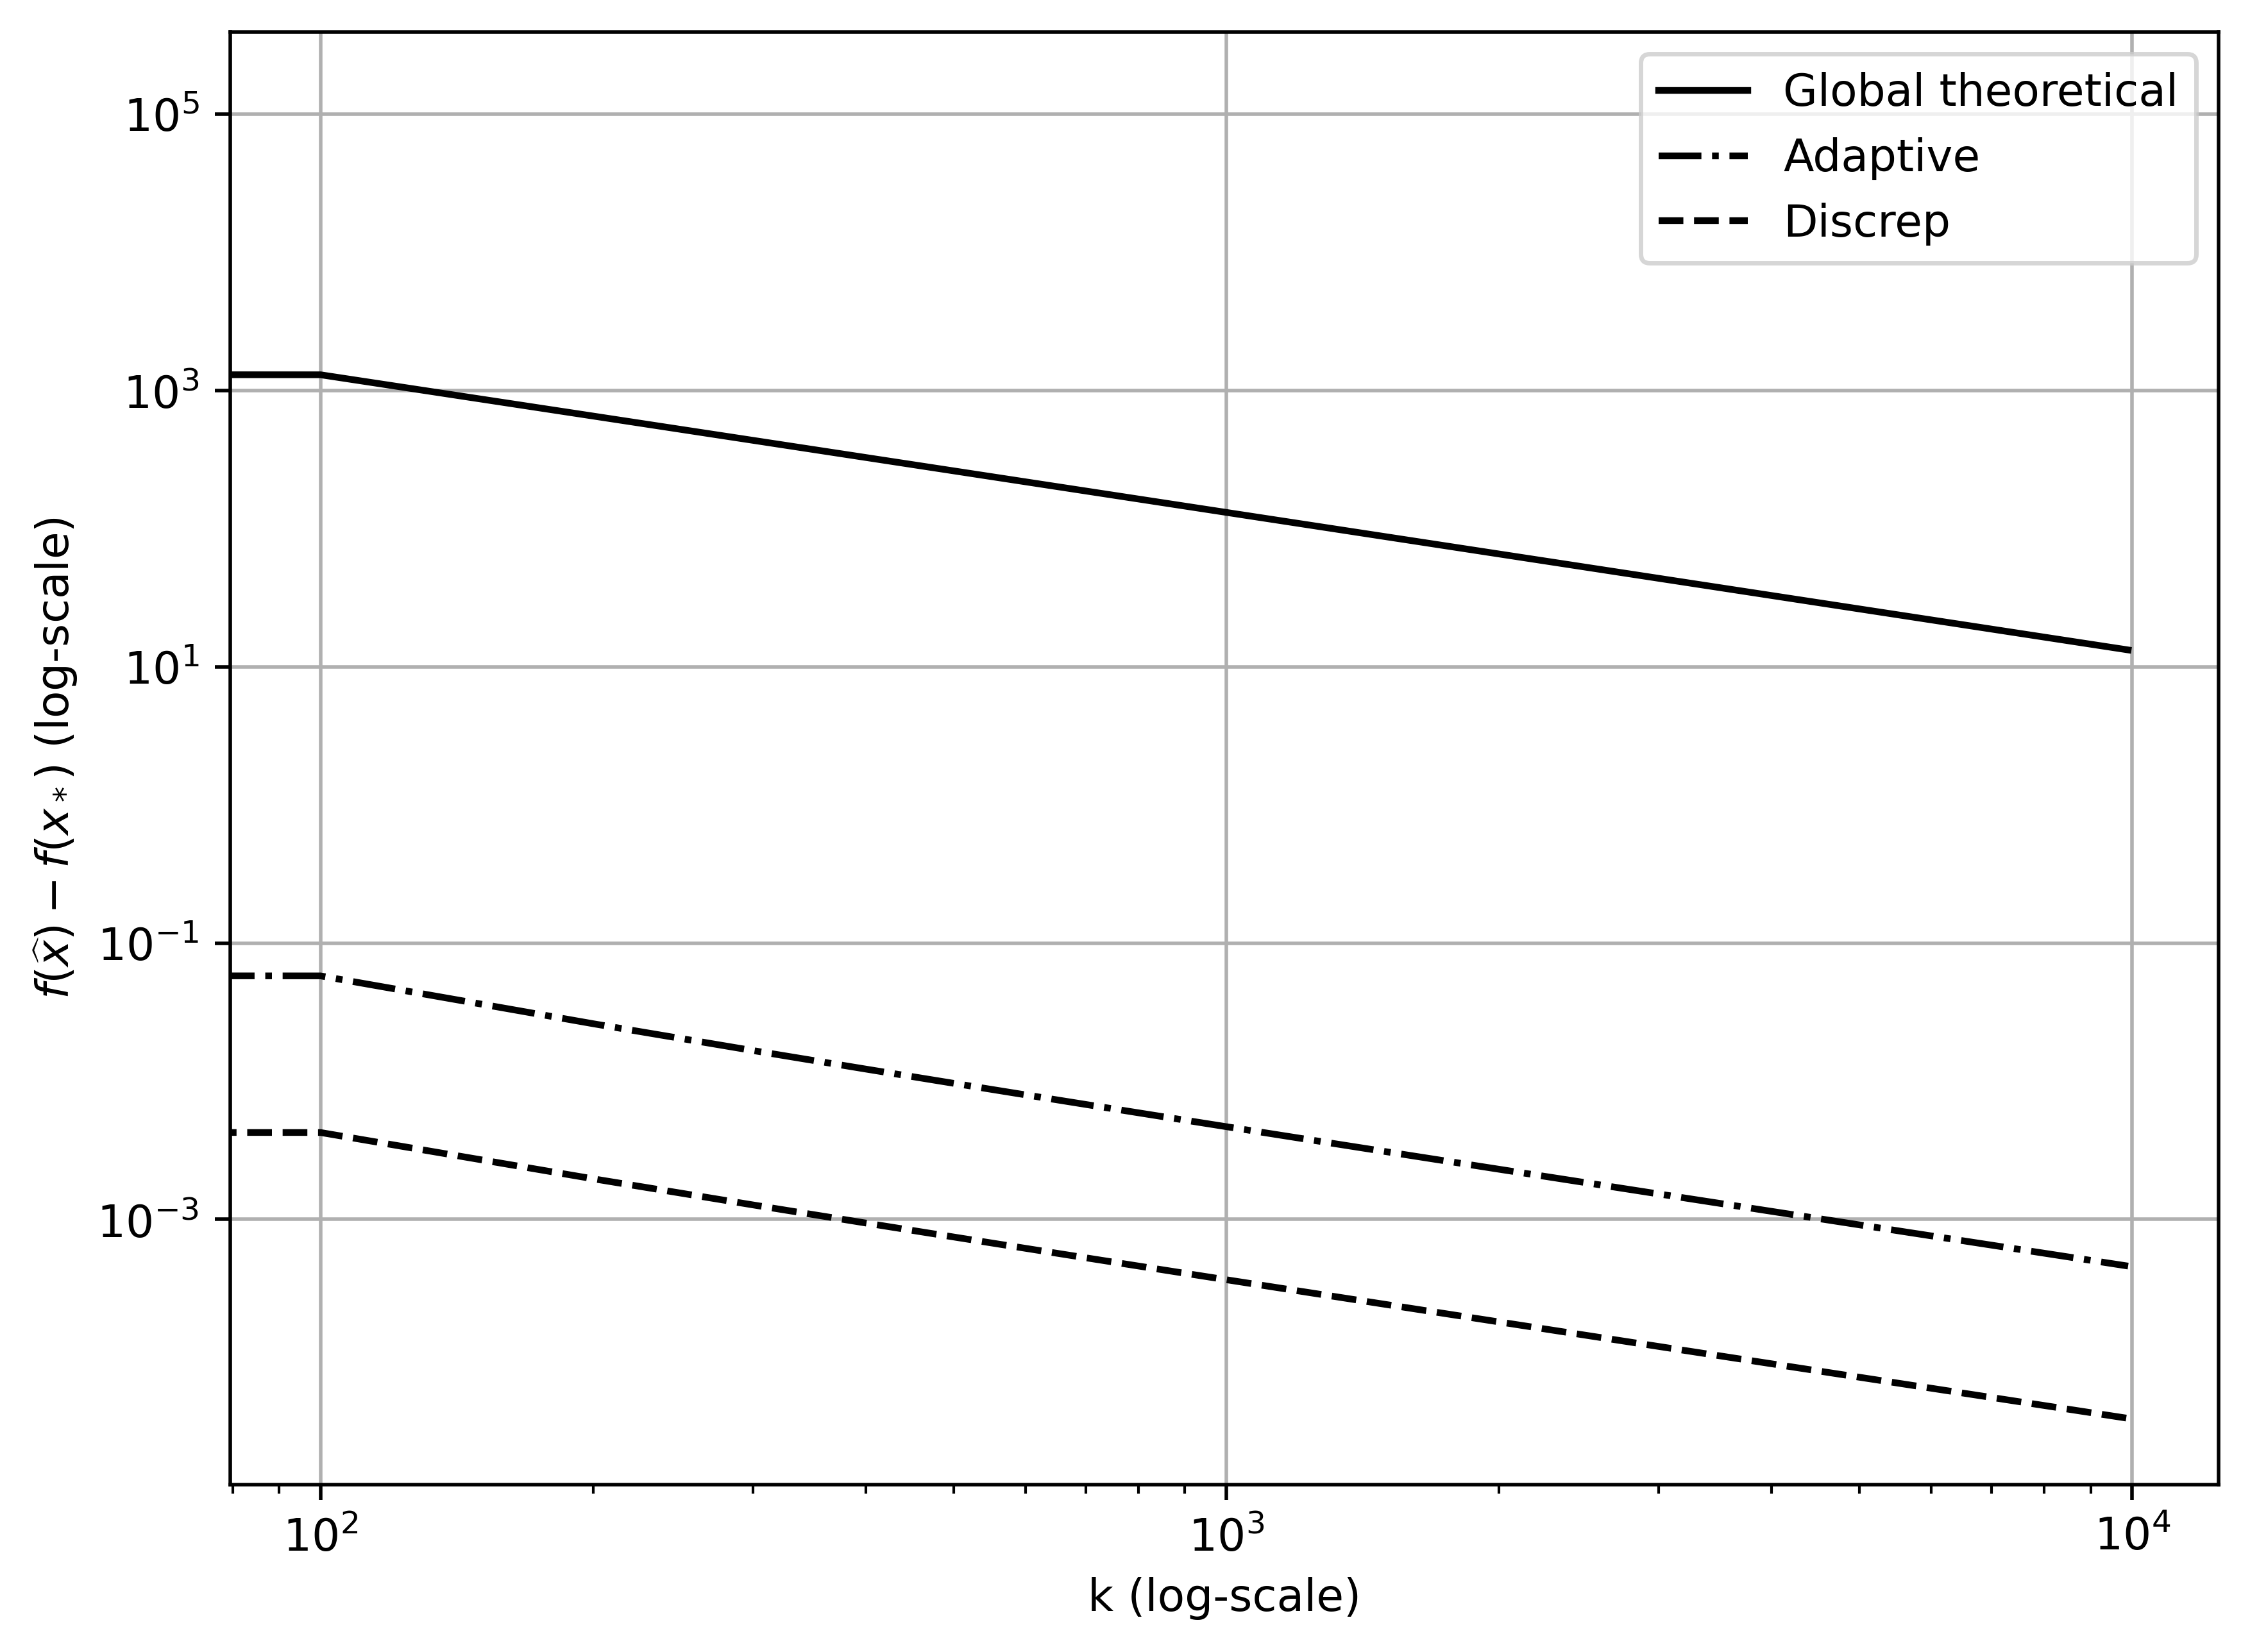
\includegraphics[width=\linewidth]{strong_convex_small_rad_f.png}
        \endminipage\hfill
        \caption{ Результаты решения задачи минимизации (\ref{sphere_cover_strongly}), где  $n= 1\,000, r = 0.7525$.}
        \label{res_strong_convex}
    \end{figure}

    Тем не менее, сравнение с известным точным решением $x_*$, а также график динамики значения целевой функции показывает, что за малое число шагов (значительно меньшее, чем для метода \eqref{orig}) реализация метода \eqref{1} приводит к неплохому качеству приближённого решения. При этом, однако, для метода, учитывающего $\Delta$-острую постановку, после достижения такого уровня дальнейшее повышение качества выходной точки в отличие от метода \eqref{orig} уже не наблюдается. 

    Данные результаты привели к идее объединения данных подходов для достижения лучших результатов в скорости сходимости без потери возможности уточнения.


\section{Рестарты для метода зеркального спуска для относительных липшицевых задач оптимизации с относительным гамма-ростом}\label{sec:ch3/sect3}
    Воспользуемся следующим результатом из \cite{Lu_2018}:
    \begin{theorem} \label{vanilla_mirror}
        Пусть $f$ --- является $M$-липшицевой на $Q$ относительно некоторой функции Брегмана $V_d(x, y)$ c 1-сильно выпуклой прокс-функцией $d(x)$. Тогда можно задать метод следующим образом:
        \begin{equation} \label{mirr_upd}
            x_{k+1} = \arg \min_{x \in Q} {\left[ f(x_k) + \langle \nabla f(x_k), x - x_k \rangle + \frac{1}{h_k} V_d(x, x_k)\right]},
        \end{equation}
        где $\{ h_k \}$ - последовательность размеров шагов.
        Для него справедлива следующая оценка скорости сходимости:
        \begin{equation} \label{general_est}
            \min_{0\leq k \leq N} f(x_k) - f(x) \leq \frac{\frac{1}{2} M^2 \sum_{k=0}^N h_k^2 + V(x, x_0)}{\sum_{k=0}^N h_k}
        \end{equation}
    \end{theorem}

    \begin{remark}
        Если в \eqref{mirr_upd} в формулировке теоремы \ref{vanilla_mirror} выбрать шаг следующим образом:
        \begin{equation} \label{mirr_step}
            h_{k} = \frac{\sqrt{2 V(x_*, x_0)}}{M\sqrt{N}},
        \end{equation}
        то можно выписать такую оценку скорости сходимости:
        \begin{equation} \label{mirr_est}
            f(\widehat{x_N}) - f(x_*) \leq \frac{M\sqrt{2V(x_*, x_0)}}{\sqrt{N}}
        \end{equation}
    \end{remark}
    Если функция обладает дополнительными свойствами, аналогичными <<острому минимуму>>,  то становится возможным применение техники рестартов. Используем аналог данного условия и вслед за Шапиро–Немировским (см. \cite{shapiro_2005} и \cite{shapiro_2021} ) введем  условие условие $\gamma$-роста ($\gamma > 1$):
    \begin{definition}
       $f$ --- удовлетворяет условию $\gamma$-роста тогда и только тогда:
       \begin{equation} \label{gamma-growth}
           f(x) - f(x_*) \geq \mu_{\gamma}\left(\min_{x_* \in X_*}{V(x_*,x)}\right)^{\gamma/2},
       \end{equation}
       где $X_*$ --- множество возможный решений.  
    \end{definition}
    
    В данных предположениях была сформулирована и доказана следующая теорема:
    \begin{theorem} \label{simple_restart}
        Пусть $f$ --- удовлетворяет условию $\gamma$-роста \eqref{gamma-growth} и также является $M$-липшицевой на $Q$ относительно некоторой функции Брегмана $V(x, y)$. В таком случае Алгоритм \ref{alg:rest_gamma} достигнет точности $\epsilon$ за:
        \begin{equation}
        \begin{aligned}
           N =\mathcal{O}\left(\frac{2 M^2}{\mu_{\gamma}^2} \log_2{\frac{V(x_*, x_0^0)}{\varepsilon}}\right) \text{ при } \gamma = 1, \\
           N = \mathcal{O}\left(\frac{2 M^2}{\mu_{\gamma}^2 \varepsilon^{(\gamma-1)} } \left[1 - \frac{1} {V(x_*, x_0^0)^{(\gamma - 1)}}\right]\right) \text{ при } \gamma > 1,
        \end{aligned}
        \end{equation}
        причем будут справедливы неравенства:
        \begin{equation}
           V(x_*, \widehat{x_p}) \leq \varepsilon
        \end{equation}
        и
        \begin{equation}
            f(\widehat{x_p}) - f(x_*) \leq  \langle \nabla f(\widehat{x_p}), \widehat{x_p} - x_* \rangle \leq M \sqrt{ 2 V(x_*, \widehat{x_p})} \leq M \sqrt{2 \varepsilon}.  
        \end{equation}
    \end{theorem}

    \begin{algorithm}[htp]
        \caption{Рестарты зеркального спуска при условии $\gamma$-роста.}
        \label{alg:rest_gamma}
        \KwData{$\varepsilon > 0$}
        \KwResult{$x_p$}
        $p \gets 0$\;
        $V(x_*, x_0) \gets V(x_*,x_0^0)$\;
        \While{$p > \log_2\left(\frac{V(x_*, x_0^0)}{\varepsilon}\right).$}{
            $x_{p}$ --- результат работы метода \eqref{mirr_upd} с шагом \eqref{mirr_step} и параметром $N_{p} = \frac{M^2 2^{\gamma}}{\mu_{\gamma}^2 2^{p(1 - \gamma)}} V(x_*, x_0^0)^{1 - \gamma}$\;
            $x_0 = \widehat{x_p}$\;
            $V(x_*, x_0) \gets \frac{1}{2^{p+1}}V_{0}(x_*, x_0^0)$\;
            $p=p+1$\;
        }
    \end{algorithm}

    \begin{proof}
       Объединим в систему свойство \eqref{gamma-growth} и оценку \eqref{mirr_est}. В доказательстве используется обозначение $x_m^n$, где $m - 0...N$ соответствует номеру итерации и $n - 0...p$ соответствует номеру рестарта: 
       $$
           \mu_{\gamma}(V(x_*, \widehat{x_N^0}))^{\gamma/2} \leq f(\widehat{x_N^0}) - f(x_*) \leq \frac{M\sqrt{V(x_*, x_0^0)}}{\sqrt{N}}
       $$
       $$
           \mu_{\gamma}(V(x_*, \widehat{x_N^0}))^{\gamma/2} \leq \frac{M\sqrt{V(x_*, x_0^0)}}{\sqrt{N}}
       $$
       $$
           (V(x_*, \widehat{x_N^0}))^{\gamma/2} \leq \frac{M\sqrt{V(x_*, x_0^0)}}{\mu_{\gamma}\sqrt{N}}
       $$
       $$
           V(x_*, \widehat{x_N^0}) \leq (\frac{M}{\mu_{\gamma}\sqrt{ N}})^{\frac{2}{\gamma}} (V(x_*, x_0^0))^{\frac{1}{\gamma}}
       $$
       $$
           V(x_*, \widehat{x_N^0}) \leq V(x_*, x_0^0) (\frac{M}{\mu_{\gamma}\sqrt{N}})^{\frac{2}{\gamma}} (V(x_*, x_0^0))^{\frac{1}{\gamma} - 1}
       $$
       Основываясь на полученной закономерности проведем последовательные оценки для первых нескольких запусков. Оценим необходимое количество итераций для 0 запуска:
       $$
           (\frac{M}{\mu_{\gamma}\sqrt{N}})^{\frac{2}{\gamma}} (V(x_*, x_0^0))^{\frac{1}{\gamma} - 1} \leq \frac{1}{2} 
       $$
       $$
           (\frac{M}{\mu_{\gamma}})^{\frac{2}{\gamma}} (V(x_*, x_0^0))^{\frac{1}{\gamma} - 1} \leq \frac{1}{2} N^{\frac{1}{\gamma}} 
       $$
       $$
           (\frac{M}{\mu_{\gamma}})^{\frac{2}{\gamma}} (V(x_*, x_0^0))^{\frac{1}{\gamma} - 1} \leq \frac{1}{2} N^{\frac{1}{\gamma}} 
       $$
       $$
           \frac{1}{2} N^{\frac{1}{\gamma}} \geq (\frac{M}{\mu_{\gamma}})^{\frac{2}{\gamma}} (V(x_*, x_0^0))^{\frac{1}{\gamma} - 1}  
       $$
       $$
           N \geq 2 ^ {\gamma} \frac{M^2}{\mu_{\gamma}^2} (V(x_*, x_0^0))^{1 - \gamma}  
       $$
       $$
           N \geq \frac{M^2 2^{\gamma}}{\mu_{\gamma}^2} (V(x_*, x_0^0))^{1 - \gamma}  
       $$
       Аналогично рассуждая получаем для 1-го запуска $x_0^1 = \widehat{x_N^0}$:
       $$
           V(x_*, \widehat{x_N^1}) \leq \frac{1}{2} V(x_*, x_0^1) = \frac{1}{2} V(x_*, \widehat{x_N^0}) \leq (\frac{1}{2})^2 V(x_*, x_0^0) 
       $$
       после:
       $$
           N_1 \geq \frac{M^2 2^{\gamma}}{\mu_{\gamma}^2} (V(x_*, x_0^1))^{1 - \gamma} \geq \frac{M^2 2^{\gamma}}{\mu_{\gamma}^2} (V(x_*, \widehat{x_N^0}))^{1 - \gamma} 
       $$
       при $\gamma > 1$:
       $$
           V(x_*, \widehat{x_N^0}) \leq \frac{1}{2}V(x_*, x_0^0)  
       $$
       $$
           (V(x_*, \widehat{x_N^0}))^{\gamma - 1} \leq (\frac{1}{2} V(x_*, x_0^0))^{\gamma - 1}
       $$
       $$
            (\frac{1}{2} V(x_*, x_0^0))^{1 - \gamma} \leq (V(x_*, \widehat{x_N^0}))^{1 - \gamma}
       $$
       соответственно:
       $$
           N_1 \geq \frac{M^2 2^{\gamma}}{\mu_{\gamma}^2} (V(x_*, \widehat{x_N^0}))^{1 - \gamma} \geq \frac{M^2 2^{\gamma}}{\mu_{\gamma}^2} (\frac{1}{2} V(x_*, x_0^0))^{1 - \gamma} = \frac{M^2 2^{\gamma}}{\mu_{\gamma}^2 2^{1-\gamma}} (V(x_*, x_0^0))^{1 - \gamma}
       $$
       Для 2-го запуска $x_0^2 = \widehat{x_N^1}$:
       $$
           V(x_*, \widehat{x_N^2}) \leq \frac{1}{2} V(x_*, x_0^2) \leq (\frac{1}{2})^3 V(x_*, x_0^0) 
       $$
       после:
       $$
           N_2 \geq \frac{M^2 2^{\gamma}}{\mu_{\gamma}^2} (V(x_*, x_0^2))^{1 - \gamma} = \frac{M^2 2^{\gamma}}{\mu_{\gamma}^2} (V(x_*, \widehat{x_N^1}))^{1 - \gamma} \geq \frac{M^2 2^{\gamma}}{\mu_{\gamma}^2 2^{1 - \gamma}} (V(x_*, x_0^1))^{1 - \gamma} \geq 
       $$
       $$
           \geq \frac{M^2 2^{\gamma}}{\mu_{\gamma}^2 2^{2(1 - \gamma)}} (V(x_*, x_0^0))^{1 - \gamma} 
       $$
       Наконец, для $(p-1)$-го запуска:
       \begin{equation} \label{v_seq}
           V(x_*, \widehat{x_N^{p-1}}) \leq \frac{1}{2^p} V(x_*, x_0^0)
       \end{equation}
       после:
       \begin{equation} \label{n_seq}
           N_{p-1} \geq \frac{M^2 2^{\gamma}}{\mu_{\gamma}^2 2^{(p - 1)(1 - \gamma)}} (V(x_*, x_0^0))^{1 - \gamma}
       \end{equation}
       Используя найденную зависимость \eqref{v_seq}, проведем оценку общего числа обращений к оракулу (здесь предполагается, что $\gamma > 1$ - равенство рассмотрим далее):
       \begin{equation} \label{n_p_sum}
       \begin{aligned}
           \sum_{k=1}^{p - 1} N_k \geq \frac{M^2 2^{\gamma}}{\mu_{\gamma}^2} (V(x_*, x_0^0))^{1 - \gamma} (1 + 2^{(\gamma-1)} + 2^{2(\gamma - 1)} + ... + 2^{(p-1)(\gamma - 1)}) = \\
           = \frac{M^2 2^{\gamma}}{\mu_{\gamma}^2} \frac{1 - 2^{(p-1)(\gamma-1)}}{1 - 2^{(\gamma-1)}} (V(x_*, x_0^0))^{1 - \gamma}
       \end{aligned}
       \end{equation}
       Удаленность от решения оценим, используя $V(x_*, \widehat{x_N^{p-1}})$:
       $$
           V(x_*, \widehat{x_N^{p-1}}) \leq \frac{1}{2^p} V(x_*, x_0^0) \leq \varepsilon
       $$
       $$
            2^p \geq \frac{1}{\varepsilon} V(x_*, x_0^0)
       $$
       Откуда и получаем необходимую оценку количества рестартов:
       \begin{equation} \label{p_rest}
            p \geq \log_2{\left[\frac{V(x_*, x_0^0)}{\varepsilon}\right]}
       \end{equation}
       Сопоставим \eqref{p_rest} и \eqref{n_p_sum} для общей оценки количества обращений к <<оракулу>>:
       $$
           \sum_{k=1}^{p} N_k \geq \frac{M^2 2^{\gamma}}{\mu_{\gamma}^2} \frac{1 - 2^{p(\gamma-1)}}{1 - 2^{(\gamma-1)}} (V(x_*, x_0^0))^{1 - \gamma} \geq 
       $$
       $$
           \geq \frac{M^2 2^{\gamma}}{\mu_{\gamma}^2 (1 - 2^{(\gamma-1)})} \left(1 - \frac{V(x_*, x_0^0)^{(\gamma-1)}}{\varepsilon^{(\gamma-1)}}\right) (V(x_*, x_0^0))^{1 - \gamma} =
       $$
       $$
           = \frac{M^2 2^{\gamma}}{\mu_{\gamma}^2 (2^{(\gamma-1)} - 1)} \left(\frac{V(x_*, x_0^0)^{(\gamma-1)}}{\varepsilon^{(\gamma-1)}} - 1\right) (V(x_*, x_0^0))^{1 - \gamma} = \frac{M^2 2^{\gamma}(1 - V(x_*, x_0^0)^{1 - \gamma}) }{\mu_{\gamma}^2 \varepsilon^{(\gamma-1)} (2^{(\gamma-1)} - 1)} = 
       $$
       $$
           = \frac{M^2}{\mu_{\gamma}^2 (\frac{1}{2} - \frac{1}{2^\gamma}) \varepsilon^{(\gamma-1)} } \left(1 - \frac{1} {V(x_*, x_0^0)^{(\gamma - 1)}}\right) \geq \frac{2 M^2}{\mu_{\gamma}^2 \varepsilon^{(\gamma-1)} } \left(1 - \frac{1} {V(x_*, x_0^0)^{(\gamma - 1)}}\right) 
       $$
       Отдельно рассмотрим случай, когда $\gamma = 1$:
       $$
           \sum_{k=1}^{p} N_k = \frac{2 p M^2}{\mu_{\gamma}^2} \geq \frac{2 M^2}{\mu_{\gamma}^2} \log_2{\left[\frac{V(x_*, x_0^0)}{\varepsilon}\right]}
       $$
       Таким образом получаем оценки:
       $$
           \mathcal{O} \left(\frac{2 M^2}{\mu_{\gamma}^2} \log_2{\frac{V(x_*, x_0^0)}{\varepsilon}}\right) \text{ при } \gamma = 1
       $$
       $$
           \mathcal{O} \left(\frac{M^2}{\mu_{\gamma}^2 \left(\frac{1}{2} - \frac{1}{2^\gamma}\right) \varepsilon^{(\gamma-1)} } \left[1 - \frac{1} {V(x_*, x_0^0)^{(\gamma - 1)}}\right]\right) =
       $$
       $$
           = \mathcal{O} \left(\frac{2 M^2}{\mu_{\gamma}^2 \varepsilon^{(\gamma-1)} } \left[1 - \frac{1} {V(x_*, x_0^0)^{(\gamma - 1)}}\right]\right) \text{ при } \gamma > 1
       $$
    \end{proof}
    Также, путем замены $\delta := M \sqrt{2 \varepsilon}$ в предыдущей теореме, можно сформулировать следующую теорему, уточнение:
    \begin{theorem}
        Пусть $f$ --- удовлетворяет условию $\gamma$-роста \eqref{gamma-growth} и также является $M$-липшицевой на $Q$ относительно некоторой дивергенции Брегмана $V(x, y)$. В таком случае Алгоритм \ref{alg:rest_gamma} достигнет точности $\delta$ за:
        \begin{equation}
            \begin{aligned}
               N = \mathcal{O}\left(\frac{2 M^2}{\mu_{\gamma}^2} \log_2{\frac{2 M^2 V(x_*, x_0^0)}{\delta^2}}\right) \text{ при } \gamma = 1, \\
               N = \mathcal{O}\left(\frac{2^\gamma M^{2\gamma}}{\mu_{\gamma}^2 \delta^{2(\gamma-1)} } \left[1 - \frac{1} {V(x_*, x_0^0)^{(\gamma - 1)}}\right]\right) \text{ при } \gamma > 1,
            \end{aligned}
        \end{equation}
        причем будут справедливы неравенства:
        \begin{equation}
           f(\widehat{x_p}) - f(x_*)  \leq \delta 
        \end{equation}
        и
        \begin{equation}
           V(x_*, \widehat{x_p}) \leq \frac{\delta^2}{2 M^2}.
        \end{equation}
    \end{theorem}

\section{Адаптивный вариант зеркального спуска для липшицевых задач с гамма-ростом}\label{sec:ch3/sect4}

    Для дальнейших рассуждений необходим адаптивный аналог оценки \eqref{general_est}. Воспользуемся результатом, полученным в лемме \ref{th:base}, а точнее в замечании \ref{remark4} к этой лемме. При помощи данного результата проведем замену глобальной константы $M$ на локальные значения в теореме \ref{vanilla_mirror}. Сформулируем и докажем следующее соответствующее данному подходу замечание:
    \begin{remark} \label{adapt_mirror}
        \begin{equation} \label{adapt_est}
            \min_{0\leq k \leq N} f(x_k) - f(x_*) \leq \frac{\sum_{k=0}^N h_k^2 \norm{\nabla f(x_k)}^2} {2 \sum_{k=0}^N h_k} + \frac{V(x_*, x_0) }{\sum_{k=0}^N h_k}.
        \end{equation}
    \end{remark}    

    \begin{proof}
       Пусть алгоритм \eqref{mirr_upd} отработал $N$ шагов, тогда просуммируем неравенства \eqref{base_eq} (из замечания \ref{remark4}):
       $$
           h_k (f(x_k) - f(x_*)) \leq h_k \langle g(x_k), x_k - x_* \rangle \leq \frac{h_k^2}{2} \norm{g(x_k)}^2 + V(x_*, x_k) - V(x_*, x_{k+1})
       $$
       $$
           \sum_{k=0}^N h_k (f(x_k) - f(x_*)) \leq \sum_{k=0}^N \frac{h_k^2}{2} \norm{g(x_k)}^2 + \sum_{k=0}^N (V(x_*, x_k) - V(x_*, x_{k+1}))
       $$
       $$
           \frac{\sum_{k=0}^N h_k f(x_k)} {\sum_{k=0}^N h_k} - f(x_*) \leq \frac{\sum_{k=0}^N h_k^2 \norm{g(x_k)}^2} {2 \sum_{k=0}^N h_k} + \frac{\sum_{k=0}^N (V(x_*, x_k) - V(x_*, x_{k+1}))}{\sum_{k=0}^N h_k}
       $$
       $$
           \min_{0\leq k \leq N} f(x_k) - f(x_*) \leq \frac{\sum_{k=0}^N h_k^2 \norm{g(x_k)}^2} {2 \sum_{k=0}^N h_k} + \frac{V(x_*, x_0) - V(x_*, x_N) }{\sum_{k=0}^N h_k} \leq
       $$
       $$
           \leq \frac{\sum_{k=0}^N h_k^2 \norm{g(x_k)}^2} {2 \sum_{k=0}^N h_k} + \frac{V(x_*, x_0) }{\sum_{k=0}^N h_k}
       $$
    \end{proof}

    \begin{remark}
        Если в \eqref{adapt_est} выбрать шаг следующим образом:
        \begin{equation} \label{eps_step}
            h_{k} = \frac{\varepsilon}{\norm{\nabla f(x_k)}^2},
        \end{equation}
        и воспользоваться критерием остановки:
        \begin{equation} \label{stop_crit}
            \sum_{k=0}^N \frac{1} {\norm{\nabla f(x_k)}^2} \geq \frac{2 V(x_*, x_0)}{\varepsilon^2}, 
        \end{equation}
        то скорость сходимости можно оценить так:
        \begin{equation} 
        \begin{aligned}
            \min_{0\leq k \leq N} f(x_k) - f(x_*) \leq \frac{\sum_{k=0}^N \frac{\varepsilon^2}{\norm{\nabla f(x_k)}^4} \norm{\nabla f(x_k)}^2} {2 \sum_{k=0}^N \frac{\varepsilon}{\norm{\nabla f(x_k)}^2}} + \frac{V(x_*, x_0) }{\sum_{k=0}^N \frac{\varepsilon}{\norm{\nabla f(x_k)}^2}} = \\
            = \frac{\varepsilon} {2} \frac{ \sum_{k=0}^N \frac{1}{\norm{\nabla f(x_k)}^2}} {\sum_{k=0}^N \frac{1} {\norm{\nabla f(x_k)}^2}} + \frac{V(x_*, x_0) }{\varepsilon \sum_{k=0}^N \frac{1} {\norm{\nabla f(x_k)}^2}}  = \frac{\varepsilon}{2} + \frac{V(x_*, x_0) }{\varepsilon \sum_{k=0}^N \frac{1} {\norm{\nabla f(x_k)}^2}} \leq \varepsilon.
        \end{aligned}
        \end{equation}
     \end{remark}
     В дальнейших рассуждениях будем обозначать 
     \[
        x_{min}^j  := \min_{0\leq k \leq N} f(x_k) \;\;\; \text{на} \;\; j\text{-м рестарте}.
     \]

     \begin{algorithm}[htp]
        \caption{Рестарты зеркального спуска при условии $\gamma$-роста с критерием остановки.}
        \label{alg:rest_criteria}
        \KwData{$\varepsilon > 0$}
        \KwResult{$x_p$}
        $p \gets 0$\;
        $V(x_*, x_0) \gets V(x_*,x_0^0)$\;
        \While{$p = \log_2{\left[\left(\frac{\mu_{\gamma}}{\varepsilon}\right)^{\frac{2}{\gamma}} \frac{V(x_*, x_0^0)}{2}\right]}.$}{
            $x_{p}$ --- результат работы метода \eqref{mirr_upd} с шагом \eqref{eps_step} и критерием остановки $\sum_{k=0}^{N_p} \frac{1}{\norm{\nabla f(x_k) }_2^2} \geq  \frac{2 \cdot 2^{\gamma} \cdot 2^{p\gamma} V(x_*, x_0) }{\mu_{\gamma}^2 V(x_*, x_0^0)^{\gamma}}  $\;
            $x_0 = x_{min}^p$\;
            $p=p+1$\;
        }
    \end{algorithm}
    \begin{theorem}
        Пусть $f$ --- удовлетворяет условию $\gamma$-роста \eqref{gamma-growth} и также является $M$-липшицевой на $Q$ относительно некоторой функции Брегмана $V_d(x, y)$. В таком случае Алгоритм \ref{alg:rest_criteria} достигнет точности $\varepsilon$ за:
        \begin{equation}
           N = \mathcal{O}\left(\frac{4 M^2}{\mu_{\gamma}^2} \log_2{\left[\left(\frac{\mu_{\gamma}}{\varepsilon}\right)^{\frac{2}{\gamma}} \frac{V(x_*, x_0^0)}{2}\right]}\right) \text{ при } \gamma = 1
       \end{equation}
       или
       \begin{equation}
           N = \mathcal{O}\left(\frac{8  M^2}{\mu_{\gamma}^2 (2 - 2^{\gamma})} \left[ \left(\frac{2}{V(x_*, x_0^0)}\right)^{(\gamma - 1)}  - \left(\frac{\mu_{\gamma}}{\varepsilon}\right)^{\frac{2\gamma - 2}{\gamma}} \right]\right) \text{ при } \gamma > 1.
       \end{equation}
    \end{theorem}

    \begin{proof}
       Поскольку начальный $\varepsilon_0$ является произвольным - выберем его следующим образом:
       \[
           \mu_{\gamma}(V(x_*, x_{min}^0))^{\frac{\gamma}{2}} \leq f(x_{min}^0) - f(x_*) \leq \varepsilon_0 \leq \mu_{\gamma}\left(\frac{V(x_*, x_0^0)}{2}\right)^{\gamma/2}
       \]
       \[
           \varepsilon_0 = \mu_{\gamma}\left(\frac{V(x_*, x_0^0)}{2}\right)^{\frac{\gamma}{2}}
       \]
       Такой выбор $\varepsilon_0$ не нарушает требований по заданной точности $\varepsilon$. Метод выстроен так, что можно показать следующее:
       \[
           \varepsilon_0 = \varepsilon \cdot \left(\sqrt{2}\right)^{p\gamma}
       \]
       Критерий остановки:
       \begin{equation} \label{krit}
           V(x_*, x_0^0) \leq \frac{1}{2} \sum_{k=0}^N \frac{\varepsilon_0^2}{\norm{\nabla f(x_k) }_2^2} \leq \frac{\mu_{\gamma}^2}{2} \frac{V(x_*, x_0^0)^{\gamma}}{2^\gamma} \sum_{k=0}^N \frac{1}{\norm{\nabla f(x_k) }_2^2}
       \end{equation}
       Если $\norm{\nabla f(x_k) }_2 \leq M$, то
       \[
           \sum_{k=0}^{N_0} \frac{1}{\norm{\nabla f(x_k) }_2^2} \geq \frac{N_0}{M^2}
       \]
       Значит критерий остановки \eqref{krit} будет заведомо выполнен при:
       \[
           V(x_*, x_0^0) \leq \frac{\mu_{\gamma}^2}{2} \frac{V(x_*, x_0^0)^{\gamma}}{2^\gamma} \frac{N_0}{M^2} \leq \frac{\mu_{\gamma}^2}{2} \frac{V(x_*, x_0^0)^{\gamma}}{2^\gamma} \sum_{k=0}^N \frac{1}{\norm{\nabla f(x_k) }_2^2}
       \]
       Откуда:
       \[
           N_0 \geq \frac{2^{\gamma + 1} M^2}{\mu_{\gamma}^2} V(x_*, x_0^0)^{(1 - \gamma)}
       \]
       Пусть:
       \[
           \varepsilon_p = \mu_{\gamma} (\frac{V(x_*, x_0^0)}{2^{p+1}})^{\frac{\gamma}{2}}
       \]
       тогда аналогично: 
       \[
           \mu_{\gamma}(V(x_*, x_{min}^p))^{\frac{\gamma}{2}} \leq f(x_{min}^p) - f(x_*) \leq \varepsilon_p
       \]
       соответственно:
       \[
           \mu_{\gamma}(V(x_*, x_{min}^{p-1}))^{\frac{\gamma}{2}} \leq \mu_{\gamma} (\frac{V(x_*, x_0^0)}{2^p})^{\frac{\gamma}{2}}
       \]
       \[  % \label{eq:v_sup}
           V(x_*, x_{min}^{p-1}) = V(x_*, x_0^p) \leq \frac{V(x_*, x_0^0)}{2^p}
       \]
       Соответствующий критерий остановки:
       \[
           V(x_*, x_0^p) \leq \frac{1}{2} \sum_{k=0}^N \frac{\varepsilon_p^2}{\norm{\nabla f(x_k) }_2^2} \leq \frac{\mu_{\gamma}^2}{2} \frac{V(x_*, x_0^0)^{\gamma}}{2^{\gamma} 2^{p\gamma}} \sum_{k=0}^{N_p} \frac{1}{\norm{\nabla f(x_k) }_2^2}
       \]
       и заведомо выполнен при:
       \[
           V(x_*, x_0^p) \leq \frac{\mu_{\gamma}^2}{2} \frac{V(x_*, x_0^0)^{\gamma}}{2^{\gamma} 2^{p\gamma}} \frac{N_p}{M^2} \leq \frac{\mu_{\gamma}^2}{2} \frac{V(x_*, x_0^0)^{\gamma}}{2^{\gamma} 2^{p\gamma}} \sum_{k=0}^{N_p} \frac{1}{\norm{\nabla f(x_k) }_2^2}
       \]
       \[
           N_p \geq \frac{2 \cdot 2^{\gamma} \cdot 2^{p\gamma} M^2}{2^p \mu_{\gamma}^2} V(x_*, x_0^0)^{(1 - \gamma)} \geq \frac{2 \cdot 2^{\gamma} \cdot 2^{p\gamma} M^2}{\mu_{\gamma}^2} \frac{V(x_*, x_0^p)}{V(x_*, x_0^0)^\gamma}
       \]
       Используя полученное неравенство мы получаем следующую оценку для $N_p$:
       \[
            N_p \geq \frac{2 \cdot 2^{\gamma} \cdot 2^{p\gamma} M^2}{2^p \mu_{\gamma}^2} V(x_*, x_0^0)^{(1 - \gamma)}
       \]
       Используя данный подход получим следующую оценку (достаточно завышенную):
       \[
        \begin{aligned}
           \sum_{k=1}^{p} N_k \geq \frac{2 \cdot 2^{\gamma} M^2}{\mu_{\gamma}^2} V(x_*, x_0^0)^{(1 - \gamma)} (1 + 2^{(\gamma-1)} + 2^{2(\gamma - 1)} + ... + 2^{p(\gamma - 1)}) = \\
           = \frac{2 \cdot 2^{\gamma} M^2}{\mu_{\gamma}^2} \frac{1 - 2^{p(\gamma-1)}}{1 - 2^{(\gamma-1)}} (V(x_*, x_0^0))^{1 - \gamma}
       \end{aligned}
       \]
       Так же отдельно рассмотрим случай $\gamma = 1$:
       \[
           \sum_{k=1}^{p} N_k = \frac{4 p M^2}{\mu_{\gamma}^2} 
       \]
       Для финальной оценки необходимо получить оценку для количества рестартов $p$, обозначим $\varepsilon := \varepsilon_p$ - то есть финальную, необходимую точность:
       \[
           \varepsilon = \varepsilon_p = \mu_{\gamma} \left(\frac{V(x_*, x_0^0)}{2^{p+1}}\right)^{\frac{\gamma}{2}}
       \]
       \[
           \left(\frac{\varepsilon}{\mu_{\gamma}}\right)^{\frac{2}{\gamma}} =  \frac{V(x_*, x_0^0)}{2^{p+1}}
       \]
       \[
            2^p =  \left(\frac{\mu_{\gamma}}{\varepsilon}\right)^{\frac{2}{\gamma}} \frac{V(x_*, x_0^0)}{2}
       \]
       \[
            p = \log_2{\left[\left(\frac{\mu_{\gamma}}{\varepsilon}\right)^{\frac{2}{\gamma}} \frac{V(x_*, x_0^0)}{2}\right]}
       \]
       Соответственно при $\gamma > 1$:
       \[
       \begin{aligned}
           \sum_{k=1}^{p} N_k \geq & \frac{2 \cdot 2^{\gamma} M^2}{\mu_{\gamma}^2} \frac{1 - 2^{p(\gamma-1)}}{1 - 2^{(\gamma-1)}} (V(x_*, x_0^0))^{1 - \gamma} = \\
           =& \frac{2 \cdot 2^{\gamma} M^2}{\mu_{\gamma}^2 (1 - 2^{(\gamma-1)})} \left[1 - \left(\left(\frac{\mu_{\gamma}}{\varepsilon}\right)^{\frac{2}{\gamma}} \frac{V(x_*, x_0^0)}{2}\right) ^{(\gamma-1)}\right] V(x_*, x_0^0)^{1 - \gamma} = \\
           =& \frac{2 \cdot 2^{\gamma} M^2}{\mu_{\gamma}^2 (1 - 2^{(\gamma-1)}) 2^{(\gamma - 1)}} \left[2^{(\gamma - 1)}V(x_*, x_0^0)^{1 - \gamma}  - \left(\frac{\mu_{\gamma}}{\varepsilon}\right)^{\frac{2\gamma - 2}{\gamma}}\right] = \\ 
           =& \frac{8  M^2}{\mu_{\gamma}^2 (2 - 2^{\gamma})} \left[\left(\frac{2}{V(x_*, x_0^0)}\right)^{(\gamma - 1)}  - \left(\frac{\mu_{\gamma}}{\varepsilon}\right)^{\frac{2\gamma - 2}{\gamma}}\right] 
       \end{aligned}
       \]
       Таким образом получаем оценки:
       \[
           \mathcal{O} \left( \frac{4 M^2}{\mu_{\gamma}^2} \log_2{\left[\left(\frac{\mu_{\gamma}}{\varepsilon}\right)^{\frac{2}{\gamma}} \frac{V(x_*, x_0^0)}{2}\right]}\right) \text{ при } \gamma = 1
       \]
       \[
           \mathcal{O} \left( \frac{8  M^2}{\mu_{\gamma}^2 (2 - 2^{\gamma})} \left[ \left(\frac{2}{V(x_*, x_0^0)}\right)^{(\gamma - 1)}  - \left(\frac{\mu_{\gamma}}{\varepsilon}\right)^{\frac{2\gamma - 2}{\gamma}} \right]\right) \text{ при } \gamma > 1
       \]
       
       \iffalse
           Соответственно при $\gamma > 1$, степень $1 - \gamma$ является отрицательной, потому справедливо следующее изменение оценки \eqref{eq:v_sup}:
           \begin{equation}
               V(x_*, x_{min}^p)^{(1 - \gamma)} \geq (\frac{V(x_*, x_0^p)}{2})^{(1 - \gamma)} \geq \frac{V(x_*, x_0^0)^{(1 - \gamma)}}{2^{p(1 - \gamma)} 2^{(1 - \gamma)}}
           \end{equation}
           то есть: 
           \begin{equation}
               V(x_*, x_0^p)^{(1 - \gamma)} \geq \frac{V(x_*, x_0^0)^{(1 - \gamma)} 2^{(1-\gamma)}}{2^{p(1 - \gamma)} 2^{(1 - \gamma)}} = \frac{V(x_*, x_0^0)^{(1 - \gamma)}}{2^{p(1 - \gamma)}}
           \end{equation}
           Используя полученное неравенство мы получаем следующую оценку для $N_p$:
           \begin{equation}
                N_p \geq \frac{2^{\gamma + 1} M^2}{\mu_{\gamma}^2} V(x_*, x_0^p)^{(1 - \gamma)} \geq  \frac{2^{\gamma + 1} M^2}{\mu_{\gamma}^2} \frac{V(x_*, x_0^0)^{(1 - \gamma)}}{2^{p(1 - \gamma)}} = \frac{2 \cdot 2^{\gamma} \cdot 2^{p\gamma} M^2}{2^p \mu_{\gamma}^2} V(x_*, x_0^0)^{(1 - \gamma)}
           \end{equation}
           Используя данный подход получим следующую оценку (достаточно завышенную):
           $$
               \sum_{k=1}^{p} N_k \geq \frac{2 \cdot 2^{\gamma} M^2}{\mu_{\gamma}^2} V(x_*, x_0^0)^{(1 - \gamma)} (1 + 2^{(\gamma-1)} + 2^{2(\gamma - 1)} + ... + 2^{p(\gamma - 1)}) = \frac{2 \cdot 2^{\gamma} M^2}{\mu_{\gamma}^2} \frac{1 - 2^{p(\gamma-1)}}{1 - 2^{(\gamma-1)}} (V(x_*, x_0^0))^{1 - \gamma}
           $$
           Так же отдельно рассмотрим случай $\gamma = 1$:
           $$
               \sum_{k=1}^{p} N_k = \frac{4 p M^2}{\mu_{\gamma}^2} 
           $$
           Для финальной оценки необходимо получить оценку для количества рестартов $p$, обозначим $\varepsilon := \varepsilon_p$ - то есть финальную, необходимую точность:
           \begin{equation}
               \varepsilon = \varepsilon_p = \mu_{\gamma} (\frac{V(x_*, x_0^p)}{2})^{\frac{\gamma}{2}} \leq  \mu_{\gamma} (\frac{V(x_*, x_0^0)}{2^{p+1}})^{\frac{\gamma}{2}}
           \end{equation}
           \begin{equation}
               (\frac{\varepsilon}{\mu_{\gamma}})^{\frac{2}{\gamma}} \leq  \frac{V(x_*, x_0^0)}{2 \cdot 2^p}
           \end{equation}
           \begin{equation}
               (\frac{\varepsilon}{\mu_{\gamma}})^{\frac{2}{\gamma}} \leq  \frac{V(x_*, x_0^0)}{2 \cdot 2^p}
           \end{equation}
           Критерий?:
           \begin{equation}
               V(x_*, x_0^p) \leq \frac{1}{2} \sum_{k=0}^N \frac{\varepsilon_p^2}{\norm{\nabla f(x_k) }_2^2} \leq \frac{\varepsilon_p^2}{2} \frac{N_p}{M^2}
           \end{equation}
       \fi
    \end{proof}

    Полученный результат имеет схожие оценки с предыдущей теоремой \ref{simple_restart}, однако на практике критерий остановки значительно сокращает количество итераций, необходимых для достижения заданной точности $\varepsilon$. Также при помощи данного метода легко прогнозируется точность перед каждым рестартом метода, что удобно для контроля за правильностью работы метода. Также подобная информация позволяет переключаться между несколькими модификациями метода, чередуя не только <<эффективные>> и <<аналитические>> шаги, но и перезапуски.  
\FloatBarrier